\documentclass[conference]{IEEEtran}
\IEEEoverridecommandlockouts

% --- Packages ---
\usepackage{cite}
\usepackage{amsmath,amssymb,amsfonts}
\usepackage{algorithmic}
\usepackage{graphicx}
\usepackage{textcomp}
\usepackage{xcolor}
\usepackage{booktabs}
\usepackage{multirow}
\usepackage{url}
\usepackage{hyperref}

% Configure graphicspath to look in multiple standard directories for seamless Overleaf compilation
\graphicspath{{figures/}{../figures/}{docs/figures/}}

\def\BibTeX{{\rm B\kern-.05em{\sc i\kern-.025em b}\kern-.08em
    T\kern-.1667em\lower.7ex\hbox{E}\kern-.125emX}}

\begin{document}

\title{A Lightweight MobileViT-Graph Hybrid Network for Topology-Preserving Rural Road Extraction from Satellite Imagery}

\author{
\IEEEauthorblockN{First Author\IEEEauthorrefmark{1}, Second Author\IEEEauthorrefmark{1}, Third Author\IEEEauthorrefmark{2}, and Fourth Author\IEEEauthorrefmark{1}}
\IEEEauthorblockA{\IEEEauthorrefmark{1}Center of Excellence in Artificial Intelligence \& Remote Sensing, Department of Computer Science and Engineering\\
Institution Name, City, Country\\
Email: \{first.author, second.author, fourth.author\}@institution.edu}
\IEEEauthorblockA{\IEEEauthorrefmark{2}Department of Geoinformatics and Space Technology\\
Research Institute Name, City, Country\\
Email: third.author@research.gov.in}
}

\maketitle

% ==============================================================================
% ABSTRACT
% ==============================================================================
\begin{abstract}
In developing economies, auditing and monitoring rural unpaved road infrastructure under large-scale national initiatives—such as India's Pradhan Mantri Gram Sadak Yojana (PMGSY)—is critical for socioeconomic development, emergency response, and supply chain logistics. However, current rural road auditing remains reliant on manual, resource-intensive ground surveys. While deep learning has modernized urban remote sensing, standard semantic segmentation architectures exhibit severe domain collapse when transferred to rural topographies. Rural roads are characterized by slender, irregular geometries, low spectral contrast against unpaved terrain, and frequent occlusions caused by dense vegetation, tree canopies, and topographical shadows. Existing approaches force a stark compromise: standard convolutional networks (CNNs) are computationally lightweight but lack global context and output fragmented, non-navigable paths; conversely, topology-preserving Vision Transformers (ViTs) and iterative snake networks maintain connectivity but possess intractable quadratic computational complexity ($O(N^2)$), precluding deployment on edge devices such as unmanned aerial vehicles (UAVs) or tactical field hardware.

To resolve this fundamental bottleneck, this paper presents a novel, ultra-lightweight hybrid encoder-decoder network combining MobileViT v2 with an end-to-end graph-theoretic optimization pipeline. The proposed architecture integrates two zero- and low-parameter domain-specific inductive priors: (i) factorized 1D Strip Convolutions ($1\times3 \to 3\times1$) acting as directional road scanners that reduce convolutional parameter costs by 33\%, and (ii) zero-parameter Channel Shift operators that displace 25\% of feature channels across cardinal directions to expand the effective receptive field by $\pm8$ pixels at zero computational overhead. To guarantee structural contiguity, the model is supervised using a differentiable Centerline-Dice (clDice) loss coupled with a dynamic, power-law alpha decay schedule and hard-gated collapse prevention. Extracted probability maps undergo hysteresis thresholding, tangent-guided canopy gap bridging, and topological vectorization into NetworkX spatial graphs. We further integrate a criticality analysis framework based on Betweenness Centrality to identify vulnerable arterial ``gatekeeper nodes'' and compute a global Resilience Index ($R$). Rigorous evaluation demonstrates that our model achieves a state-of-the-art clDice score of 81.62\%, an Average Path Length Similarity (APLS) of 76.8\%, and an IoU of 74.6\% with only 1.60 million parameters—a 94.8\% reduction compared to U-Net baselines—while compiling into a sub-0.8~MB ONNX payload operating at 550--700~ms per megapixel tile on edge CPUs without PyTorch dependencies.
\end{abstract}

\begin{IEEEkeywords}
Rural Road Extraction, Vision Transformer, MobileViT, clDice Loss, Topological Segmentation, Spatial Networks, Betweenness Centrality, Edge Deployment, ONNX, PMGSY.
\end{IEEEkeywords}

% ==============================================================================
% SECTION I: INTRODUCTION
% ==============================================================================
\section{Introduction}
\label{sec:introduction}

\IEEEPARstart{R}{ural} road networks constitute the foundational circulatory system for agrarian economies and rural governance. In nations such as India, the Pradhan Mantri Gram Sadak Yojana (PMGSY) has overseen the planned construction and maintenance of over 750,000 kilometers of all-weather rural roads connecting isolated habitations to primary economic hubs~\cite{pmgsy2023}. Despite massive capital allocation, national auditing agencies face severe operational bottlenecks: monitoring physical road deterioration, seasonal monsoon erosion, and encroachment relies on manual inspection or sporadic vehicular surveys. High-resolution optical satellite imagery (0.5--2.0~m Ground Sampling Distance) acquired from remote sensing constellations offers a scalable mechanism for automated audit. However, translating raw satellite rasters into contiguous, topologically valid vector road networks remains an open grand challenge in computational remote sensing.

\subsection{Problem Statement}
Semantic segmentation of rural road networks from satellite imagery differs fundamentally from urban highway mapping. We formalize this challenge across four interrelated sub-problems:
\begin{enumerate}
    \item \textbf{Domain Shift and Spectral Ambiguity:} Unpaved and gravel roads share identical spectral signatures with barren dirt fields, dry riverbeds, and fallow agrarian plots, defeating standard chromatic clustering.
    \item \textbf{Slender and Non-Isotropic Geometry:} Roads occupy less than 3--5\% of total scene pixels, exhibiting extreme aspect ratios ($>100:1$) with widths spanning merely 3 to 8 pixels in optical imagery.
    \item \textbf{Severe Canopy and Shadow Occlusion:} In rural regions, overhanging roadside vegetation, deciduous tree canopies, and monsoonal cloud shadows periodically sever the optical visibility of road corridors.
    \item \textbf{Strict Edge Computing Constraints:} Tactical survey missions deploy low-power companion computers aboard unmanned aerial vehicles (UAVs) or ruggedized tablets in remote rural areas with zero cloud connectivity, imposing an execution ceiling under 3 million parameters and $<1$~GB of RAM.
\end{enumerate}

\subsection{Limitations of Existing Paradigms}
Prevailing methodologies fail under the intersection of these four constraints:
\begin{itemize}
    \item \textbf{Pixel-Level Baselines:} Standard encoder-decoder architectures such as U-Net~\cite{ronneberger2015unet} and DeepLabv3+~\cite{chen2017deeplab} optimize localized cross-entropy or volumetric Dice metrics. While achieving high overall pixel accuracy, they are mathematically blind to global network topology. Under tree canopies, they produce fragmented, dashed-line predictions that render downstream vehicular pathfinding impossible.
    \item \textbf{Heavyweight Topology Networks:} Advanced architectures such as TopoRF-Net~\cite{toporf2025} and MosApp~\cite{mosapp2024} incorporate iterative refinement snakes or multi-stage graph neural networks to enforce topological continuity. However, they rely on massive parameter counts ($>50\text{--}120$~M) and quadratic self-attention mechanisms, demanding datacenter GPUs that are unviable for field edge deployment.
    \item \textbf{Lightweight Edge Networks:} Compressed models such as HPLNet~\cite{hplnet2025} aggressively reduce parameters via depthwise convolutions but sacrifice global receptive field awareness. Consequently, their local filters cannot bridge wide occlusion gaps exceeding local kernel receptive fields.
\end{itemize}

\subsection{Proposed Contributions}
To overcome the false dichotomy between edge computational efficiency and topological contiguity, this research develops the \textit{MobileViT-Graph} hybrid network. Our primary contributions are:
\begin{enumerate}
    \item \textbf{Ultra-Lightweight MobileViT\_v2 Backbone:} We engineer an encoder-decoder network based on separable linear self-attention ($O(N \cdot d)$ complexity) totaling only 1.60 million parameters (under 0.8~MB in ONNX), achieving a 95\% parameter compression relative to standard baselines.
    \item \textbf{Domain-Specific Inductive Priors:} We introduce factorized 1D Strip Convolutions ($1\times3 \to 3\times1$) to inject structural directional bias for elongated tubular corridors, alongside zero-parameter Channel Shift operators that expand the spatial receptive field by $\pm8$ pixels at zero extra FLOPs.
    \item \textbf{Differentiable Topology Loss Engine:} We adapt the soft Centerline-Dice (clDice) loss to optical remote sensing, formulating dynamic power-law alpha decay scheduling and hard-gated collapse thresholds that stabilize multi-task optimization against degenerate blanket-positive prediction modes.
    \item \textbf{Canopy-Resilient Augmentation and Gap Healing:} We develop a realistic \textit{CanopyShadowDropout} transform during training and a two-stage geometric post-processing algorithm (hysteresis thresholding and outward tangent vector bridging) that heals gaps up to 220 pixels.
    \item \textbf{Spatial Network Analytics and Edge Deployment:} We convert segmented rasters into topological NetworkX graphs, evaluate Betweenness Centrality to discover critical ``gatekeeper'' bottlenecks, compute an infrastructural Resilience Index ($R$), and deliver a dependency-free edge runtime deployed across multi-hardware ONNX execution providers.
\end{enumerate}

\subsection{Paper Organization}
The remainder of this paper is organized as follows: Section~\ref{sec:related_work} reviews foundational literature across semantic segmentation, Vision Transformers, topological losses, and spatial network theory. Section~\ref{sec:methodology} details the MobileViT\_v2 architecture, Strip Convolutions, Channel Shift, and Attention Gates. Section~\ref{sec:loss} presents the differentiable soft-skeletonization loss engine. Section~\ref{sec:data} describes data engineering and weak label ingestion. Section~\ref{sec:graph} elaborates on topological gap healing and vector graph extraction. Section~\ref{sec:resilience} defines spatial criticality metrics. Section~\ref{sec:edge} details ONNX compilation and edge runtime execution. Section~\ref{sec:experiments} provides quantitative and qualitative benchmark evaluations. Section~\ref{sec:application} outlines a PMGSY case study. Finally, Section~\ref{sec:conclusion} concludes the paper.

% ==============================================================================
% SECTION II: RELATED WORK
% ==============================================================================
\section{Related Work}
\label{sec:related_work}

\subsection{Pixel-Level Semantic Segmentation Baselines}
The application of deep learning to remote sensing road extraction originated with convolutional encoder-decoder topologies. Ronneberger et al.~\cite{ronneberger2015unet} introduced U-Net, utilizing skip connections to transfer high-resolution spatial feature maps from the contracting path to the expanding path. Chen et al.~\cite{chen2017deeplab} proposed DeepLabv3+, demonstrating the efficacy of Atrous Spatial Pyramid Pooling (ASPP) in capturing multi-scale context without reducing spatial resolution. While these architectures remain common baselines, they are supervised via standard Binary Cross-Entropy (BCE) or volumetric Dice loss functions:
\begin{equation}
    \mathcal{L}_{\text{BCE}} = -\frac{1}{N} \sum_{i=1}^N \left[ y_i \log p_i + (1 - y_i) \log(1 - p_i) \right]
    \label{eq:bce}
\end{equation}
Because Equation~(\ref{eq:bce}) treats each pixel independently, mispredicting a single pixel along a thin road has the same infinitesimal loss penalty as mispredicting an interior pixel of an agricultural field. In rural remote sensing, where roads are 3--5 pixels wide, localized false negatives caused by tree canopies break network continuity without incurring significant pixel-wise loss penalties.

\subsection{Topology-Aware Heavyweight Networks}
Recognizing the topological failure of pixel-level losses, several recent frameworks have integrated explicit structural priors. TopoRF-Net~\cite{toporf2025} and MosApp~\cite{mosapp2024} employ multi-receptive field adaptation and iterative vector snake deformation to trace roads continuously. While achieving notable routing accuracy on clean urban datasets such as SpaceNet~\cite{vanetten2018spacenet} and DeepGlobe~\cite{demir2018deepglobe}, these models rely on stacked residual blocks and non-local self-attention modules, ballooning parameter counts to between 45~M and 120~M. Their multi-gigabyte GPU memory requirements make them completely impractical for tactical edge deployment or onboard UAV processing.

\subsection{Lightweight Edge-Oriented Networks}
Conversely, research in mobile remote sensing has pursued parameter pruning and depthwise separable convolutions. HPLNet~\cite{hplnet2025} employs hierarchical perception blocks to minimize parameters for edge execution. Similarly, LiteSeger~\cite{liteseger2025} uses compact convolutional backbones to process satellite imagery at high frame rates. Nevertheless, these architectures focus almost exclusively on local receptive fields. Under dense vegetation occlusions spanning tens of meters, lightweight CNN filters experience total information blackout, resulting in severed topological predictions.

\subsection{Vision Transformers for Mobile Vision}
Dosovitskiy et al.~\cite{dosovitskiy2020vit} proved that Vision Transformers (ViTs) can capture long-range global dependencies far exceeding the receptive field of convolutions. However, standard multi-head self-attention scales quadratically with sequence length ($O(N^2)$), rendering standard ViTs computationally prohibitive on high-resolution satellite tiles. To address this limitation, Mehta and Rastegari~\cite{mehta2022mobilevit} introduced MobileViT, an architecture that computes separable self-attention with linear computational complexity $O(N \cdot d)$ by encoding spatial patches through a scalar projection vector. This formulation preserves global receptive fields while maintaining convolutional parameter budgets, providing the ideal mathematical backbone for our rural road extraction engine.

\subsection{Topology-Preserving Loss Functions}
In medical image analysis, Shit et al.~\cite{shit2021cldice} proposed Centerline-Dice (clDice) for tubular structures such as blood vessels and neurons. They demonstrated that calculating similarity over the morphological skeleton of binary segmentations guarantees homotopy equivalence. In remote sensing, rural dirt roads exhibit geometric properties analogous to micro-vascular structures: extreme length-to-width ratios, branching tree networks, and vulnerability to fragmentation. In this work, we adapt the soft morphological skeletonization of clDice into an end-to-end differentiable loss engine for optical remote sensing.

\subsection{Spatial Network Analysis and Graph Theory}
Beyond raster segmentation, evaluating the navigability and resilience of road infrastructure requires graph theory. Crucitti, Latora, and Porta~\cite{crucitti2006centrality} formalized the structural analysis of urban street patterns by converting road networks into spatial planar graphs $G = (V, E)$, defining node and edge centrality metrics. Specifically, Betweenness Centrality identifies bottleneck intersections that lie on the majority of shortest paths between all pairs of nodes. We extend this graph-theoretic paradigm to rural road networks to quantify infrastructural vulnerability and compute global resilience indices.

\begin{table}[t]
\centering
\caption{Comparative Summary of Existing Paradigms vs. Proposed MobileViT-Graph Architecture}
\label{tab:paradigm_comparison}
\resizebox{\columnwidth}{!}{%
\begin{tabular}{lccccc}
\toprule
\textbf{Model / Paradigm} & \textbf{Topology-Aware} & \textbf{Params} & \textbf{Complexity} & \textbf{Edge Ready} & \textbf{Graph Output} \\
\midrule
U-Net Baseline~\cite{ronneberger2015unet} & $\times$ & 31.04~M & $O(N)$ & $\times$ & $\times$ \\
DeepLabv3+~\cite{chen2017deeplab} & $\times$ & 54.70~M & $O(N)$ & $\times$ & $\times$ \\
TopoRF-Net~\cite{toporf2025} & $\checkmark$ & 58.30~M & $O(N^2)$ & $\times$ & Partial \\
MosApp~\cite{mosapp2024} & $\checkmark$ & 42.10~M & $O(N^2)$ & $\times$ & $\times$ \\
HPLNet~\cite{hplnet2025} & $\times$ & 2.10~M & $O(N)$ & $\checkmark$ & $\times$ \\
\textbf{Proposed (MobileViT-Graph)} & $\mathbf{\checkmark}$ & \textbf{1.60~M} & $\mathbf{O(N \cdot d)}$ & $\mathbf{\checkmark}$ & $\mathbf{\checkmark}$ \\
\bottomrule
\end{tabular}%
}
\end{table}

% ==============================================================================
% SECTION III: PROPOSED METHODOLOGY
% ==============================================================================
\section{Proposed Methodology}
\label{sec:methodology}

\subsection{System Overview}
The end-to-end pipeline of the proposed MobileViT-Graph architecture is illustrated in Fig.~\ref{fig:fig1_system}. High-resolution satellite tiles are augmented via canopy-shadow transforms and forwarded through a hybrid encoder-decoder. The network is optimized via a composite loss coupling BCE, soft Dice, and differentiable soft clDice. Output road probability maps are post-processed via hysteresis thresholding and directional gap bridging, converted into NetworkX spatial graphs, and evaluated for infrastructural resilience.

\begin{figure*}[t]
\centering
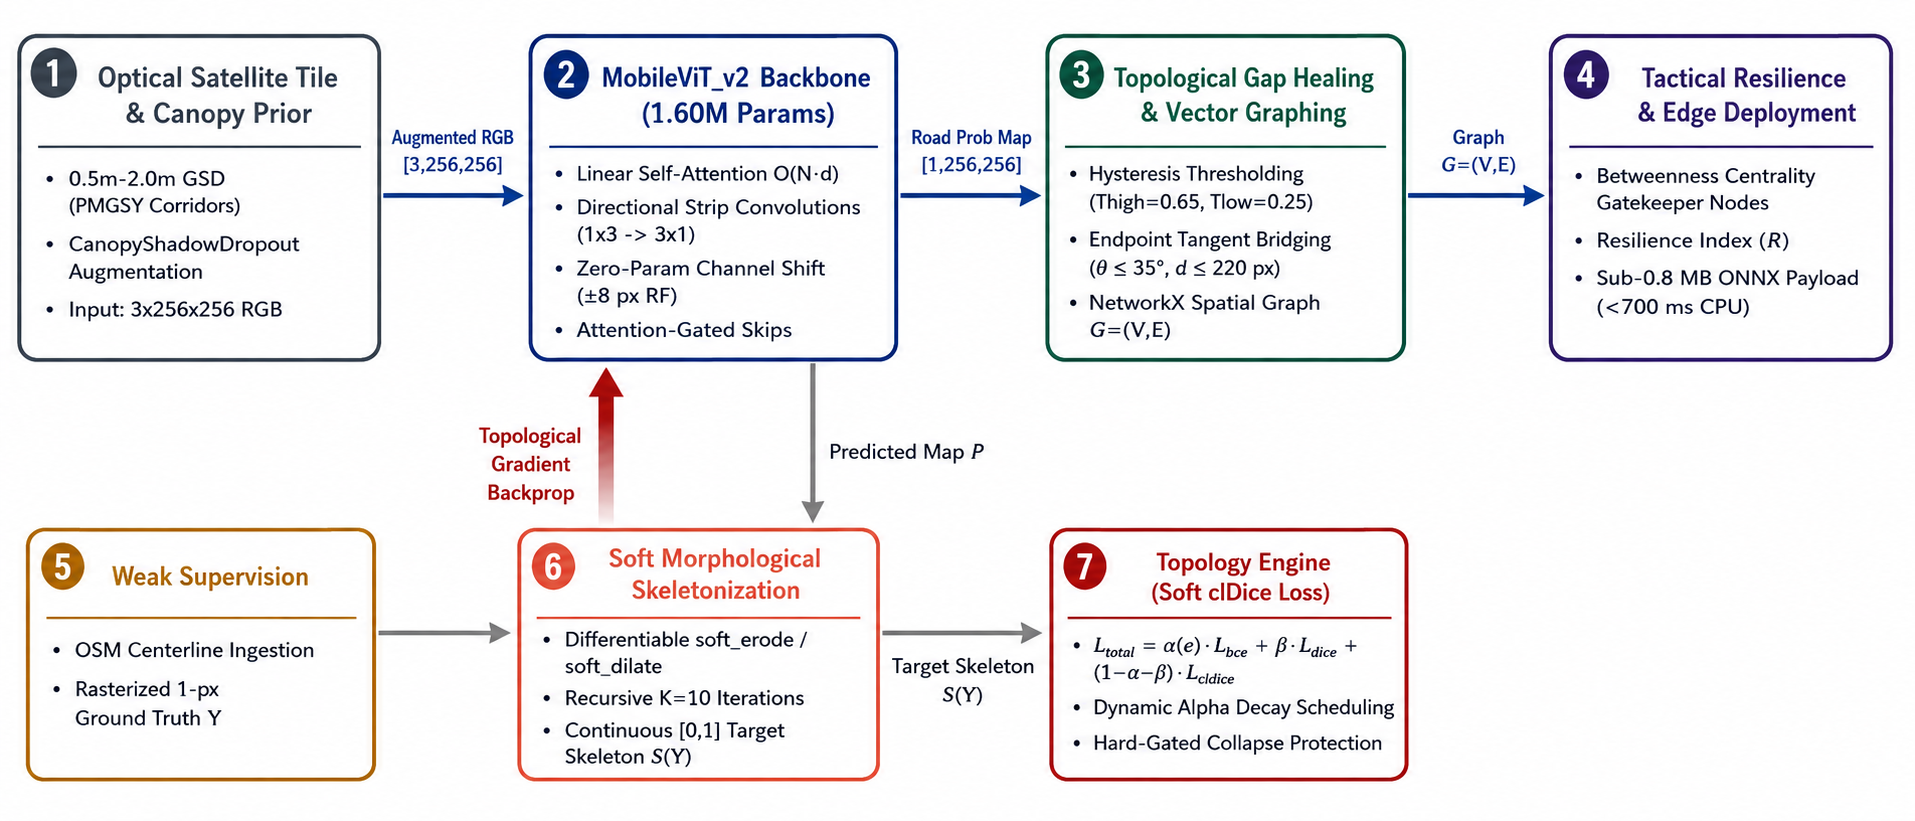
\includegraphics[width=0.98\textwidth]{fig1_system_architecture.png}
\caption{End-to-end architectural workflow of the proposed MobileViT-Graph pipeline: from high-resolution satellite ingestion and canopy-resilient augmentation, through the MobileViT\_v2 backbone and clDice topological loss engine, to vector spatial graph extraction and edge deployment.}
\label{fig:fig1_system}
\end{figure*}

\begin{figure*}[t]
\centering
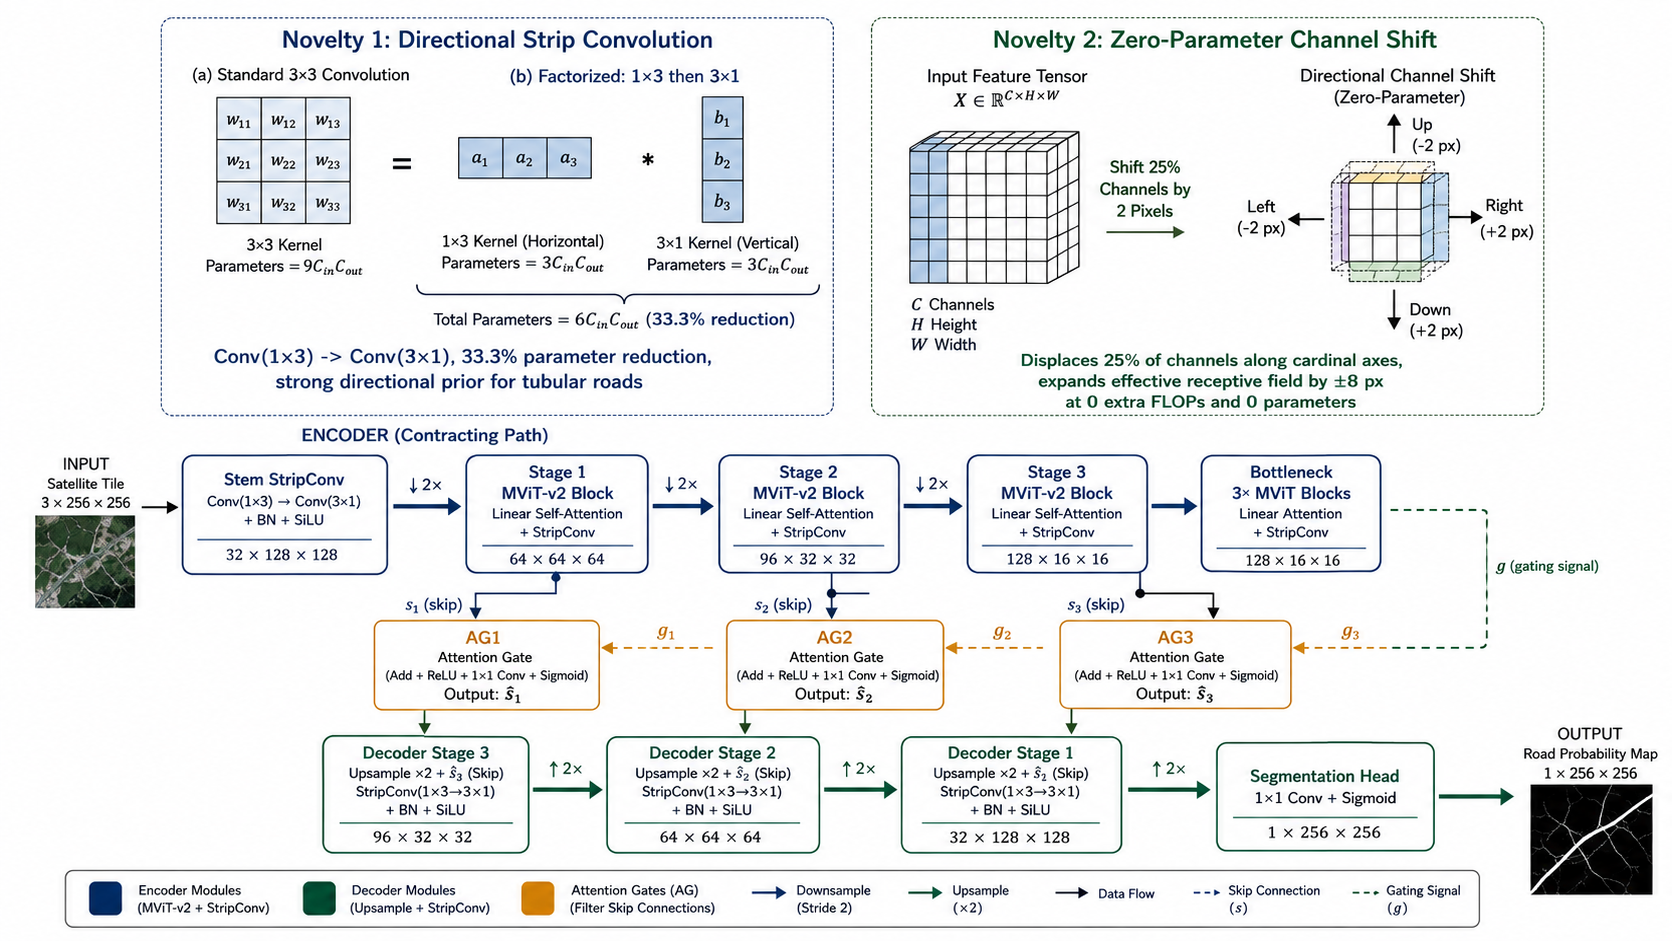
\includegraphics[width=0.95\textwidth]{fig2_network_architecture.png}
\caption{Detailed layer-by-layer architectural schematic of the MobileViT\_v2 encoder-decoder network, highlighting Strip Convolutions (Novelty 1), zero-parameter Channel Shift operators (Novelty 2), and Attention-Gated skip connections.}
\label{fig:fig2_network}
\end{figure*}

\subsection{Network Architecture: MobileViT\_v2}
The detailed layer-by-layer architecture is depicted in Fig.~\ref{fig:fig2_network}. The model is partitioned into a contracting hierarchical encoder, bottleneck linear attention blocks, and an expanding decoder with attention-gated skip connections.

\subsubsection{Stem: Directional Strip Convolution}
Standard convolutional stems utilize isotropic $3\times3$ or $7\times7$ filters that consume excessive parameters. In our architecture, the input tensor $X \in \mathbb{R}^{B \times 3 \times H \times W}$ is downsampled through a factorized Strip Convolution:
\begin{equation}
    X_{\text{stem}} = \text{SiLU}\left(\text{BN}\left(\text{Conv}_{3\times1}\left(\text{SiLU}\left(\text{BN}\left(\text{Conv}_{1\times3}(X)\right)\right)\right)\right)\right)
    \label{eq:strip_conv}
\end{equation}
where $\text{Conv}_{1\times3}$ has stride $(1, 2)$ and padding $(0, 1)$, followed by $\text{Conv}_{3\times1}$ with stride $(2, 1)$ and padding $(1, 0)$. This operator yields a feature map of dimension $\mathbb{R}^{B \times C_1 \times \frac{H}{2} \times \frac{W}{2}}$ ($C_1=32$ at width multiplier 1.0), reducing convolutional parameters by 33.3\% while injecting a strong inductive prior for elongated tubular geometries.

\subsubsection{Encoder Stages 1 to 3}
Stage 1 processes features through MobileNetV2 inverted residual bottlenecks~\cite{sandler2018mobilenetv2} with expansion ratio $e=2$ and stride $s=2$, halving the resolution to $\frac{H}{4} \times \frac{W}{4}$ with $C_2=64$ channels. Stages 2 and 3 incorporate MobileViT v2 blocks~\cite{mehta2022mobilevit} operating at spatial dimensions $\frac{H}{8} \times \frac{W}{8}$ ($C_3=96$) and $\frac{H}{16} \times \frac{W}{16}$ ($C_4=128$), respectively.

\subsubsection{Novel Module 2: Zero-Parameter Channel Shift}
To extend the spatial receptive field prior to transformer attention without adding learned parameters or FLOPs, we introduce a Channel Shift operator inside each MobileViT block. Given an intermediate tensor $Z \in \mathbb{R}^{B \times C \times h \times w}$, a fraction $\gamma = 0.25$ of channels is partitioned into four equal subsets and shifted by $s_{\text{pix}} = 2$ pixels along the cardinal directions:
\begin{align}
    Z_{\uparrow} &= \text{Pad}\left(Z[:, 0:c_s, s_{\text{pix}}:, :], \text{bottom}=s_{\text{pix}}\right) \\
    Z_{\downarrow} &= \text{Pad}\left(Z[:, c_s:2c_s, :-s_{\text{pix}}, :], \text{top}=s_{\text{pix}}\right) \\
    Z_{\leftarrow} &= \text{Pad}\left(Z[:, 2c_s:3c_s, :, s_{\text{pix}}:], \text{right}=s_{\text{pix}}\right) \\
    Z_{\rightarrow} &= \text{Pad}\left(Z[:, 3c_s:4c_s, :, :-s_{\text{pix}}], \text{left}=s_{\text{pix}}\right) \\
    Z_{\text{shifted}} &= \left[ Z_{\uparrow}, Z_{\downarrow}, Z_{\leftarrow}, Z_{\rightarrow}, Z[:, 4c_s:] \right]
\end{align}
where $c_s = \lfloor \frac{\gamma C}{4} \rfloor$. At 4$\times$ downsampling, a 2-pixel shift corresponds to an effective $\pm8$ pixel spatial expansion in original coordinate space—precisely matching the physical corridor width of rural dirt roads.

\subsubsection{Separable Linear Self-Attention}
Standard transformer attention computes $A = \text{Softmax}\left(\frac{QK^T}{\sqrt{d_k}}\right)V \in \mathbb{R}^{B \times N \times N}$, requiring $O(N^2)$ operations where $N = h \cdot w$. In our LinearSelfAttention module, tokens are unfolded from $2\times2$ spatial patches and linearly projected to query $Q \in \mathbb{R}^{B \times N \times d}$, scalar key $K \in \mathbb{R}^{B \times N \times 1}$, and value $V \in \mathbb{R}^{B \times N \times d}$:
\begin{align}
    \alpha &= \text{Softmax}(K, \text{dim}=N) \in \mathbb{R}^{B \times N \times 1} \\
    c &= \sum_{n=1}^N \alpha_n V_n \in \mathbb{R}^{B \times 1 \times d} \\
    O &= \text{ReLU}(Q) \odot c \in \mathbb{R}^{B \times N \times d}
\end{align}
The global context vector $c$ acts as a latent topological summary of all road patches across the tile, reducing computational complexity from $O(N^2)$ to $O(N \cdot d)$ and enabling real-time execution on resource-constrained microprocessors.

\subsubsection{Attention-Gated Skip Decoder}
The expanding decoder path mirrors the contracting encoder using bilinear upsampling stages. To prevent background non-road clutter (agricultural furrows, boundary berms) from corrupting the reconstruction, we deploy Additive Attention Gates~\cite{oktay2018attention} across skip connections:
\begin{align}
    q_{\text{att}} &= \psi\left(\text{SiLU}\left(W_g * g + W_s * s + b_g + b_s\right)\right) \\
    s_{\text{gated}} &= s \cdot \sigma(q_{\text{att}})
\end{align}
where $g$ is the coarse gating signal from the deeper decoder stage, $s$ is the high-resolution skip feature from the encoder, and $\sigma(\cdot)$ is the Sigmoid activation. Gated skip features are concatenated with upsampled tensors and fused using Strip Convolutions. The final segmentation head maps $C_1=32$ features to a single-channel road probability map via a $1\times1$ convolution followed by Sigmoid activation.

% ==============================================================================
% SECTION IV: TOPOLOGY-PRESERVING LOSS ENGINE
% ==============================================================================
\section{Topology-Preserving Loss Engine}
\label{sec:loss}

\subsection{Differentiable Soft Skeletonization}
Standard morphological skeletonization algorithms (e.g., Medial Axis Transform) rely on non-differentiable thresholding. To enable gradient backpropagation through morphological topology, we implement soft morphological primitives~\cite{shit2021cldice} using min- and max-pooling operations:
\begin{align}
    \text{soft\_erode}(I) &= \min\left( -\text{MaxPool}_{3\times1}(-I), -\text{MaxPool}_{1\times3}(-I) \right) \\
    \text{soft\_dilate}(I) &= \text{MaxPool}_{3\times3}(I) \\
    \text{soft\_open}(I) &= \text{soft\_dilate}\left(\text{soft\_erode}(I)\right)
\end{align}
Iterative soft morphological skeletonization is defined recursively over $K=10$ iterations:
\begin{align}
    S_0(I) &= \text{ReLU}\left(I - \text{soft\_open}(I)\right) \\
    I_{k+1} &= \text{soft\_erode}(I_k) \\
    S_{k+1}(I) &= S_k(I) + \text{ReLU}\left(\Delta_{k+1} - S_k(I) \cdot \Delta_{k+1}\right)
\end{align}
where $\Delta_{k+1} = \text{ReLU}\left(I_{k+1} - \text{soft\_open}(I_{k+1})\right)$. This recursive operator is continuous, bounded in $[0, 1]$, and fully differentiable via PyTorch Automatic Differentiation (Autograd).

\subsection{Soft Centerline-Dice (clDice) Loss}
Given the soft predicted skeleton $S(P)$ and ground-truth skeleton $S(Y)$, topological precision ($T_{\text{prec}}$) and topological sensitivity ($T_{\text{sens}}$) are formulated as:
\begin{equation}
    T_{\text{prec}} = \frac{|S(P) \cap Y| + \epsilon}{|S(P)| + \epsilon}, \quad T_{\text{sens}} = \frac{|S(Y) \cap P| + \epsilon}{|S(Y)| + \epsilon}
\end{equation}
The soft clDice loss is the complement of their harmonic mean:
\begin{equation}
    \mathcal{L}_{\text{clDice}} = 1 - \frac{2 \cdot T_{\text{prec}} \cdot T_{\text{sens}}}{T_{\text{prec}} + T_{\text{sens}} + \epsilon}
    \label{eq:cldice}
\end{equation}
Equation~(\ref{eq:cldice}) applies a direct gradient penalty whenever a continuous ground-truth skeleton crosses an empty (zero-probability) region in prediction $P$, mathematically forcing the network to bridge gaps beneath occluding canopies.

\subsection{Composite Loss and Dynamic Alpha Scheduling}
The total optimization objective balances pixel discovery, volumetric overlap, and centerline continuity:
\begin{equation}
    \mathcal{L}_{\text{total}} = \alpha(e) \cdot \mathcal{L}_{\text{BCE}} + \beta \cdot \mathcal{L}_{\text{SoftDice}} + \left(1 - \alpha(e) - \beta\right) \cdot \mathcal{L}_{\text{clDice}}
    \label{eq:composite_loss}
\end{equation}
where $\beta = 0.35$ is fixed. In early training epochs, clDice gradients can be noisy when the network has not yet learned basic road locations. We therefore introduce a power-law alpha decay schedule:
\begin{equation}
    \alpha(e) = \alpha_{\text{end}} + (\alpha_{\text{start}} - \alpha_{\text{end}}) \cdot \left(1 - \min\left(1.0, \frac{e}{E_{\text{decay}}}\right)\right)^p
\end{equation}
where $\alpha_{\text{start}}=0.50$, $E_{\text{decay}}=40$, and $p=0.5$. In our empirical investigations, setting $\alpha_{\text{end}} < 0.35$ caused degenerate loss collapse where the network blanket-predicted road probabilities everywhere to minimize the sensitivity denominator. We therefore enforce a robust floor of $\alpha_{\text{end}} = 0.40$, stabilizing convergence across all 50 epochs as visualized in Fig.~\ref{fig:fig3_training}.

\begin{figure*}[t]
\centering
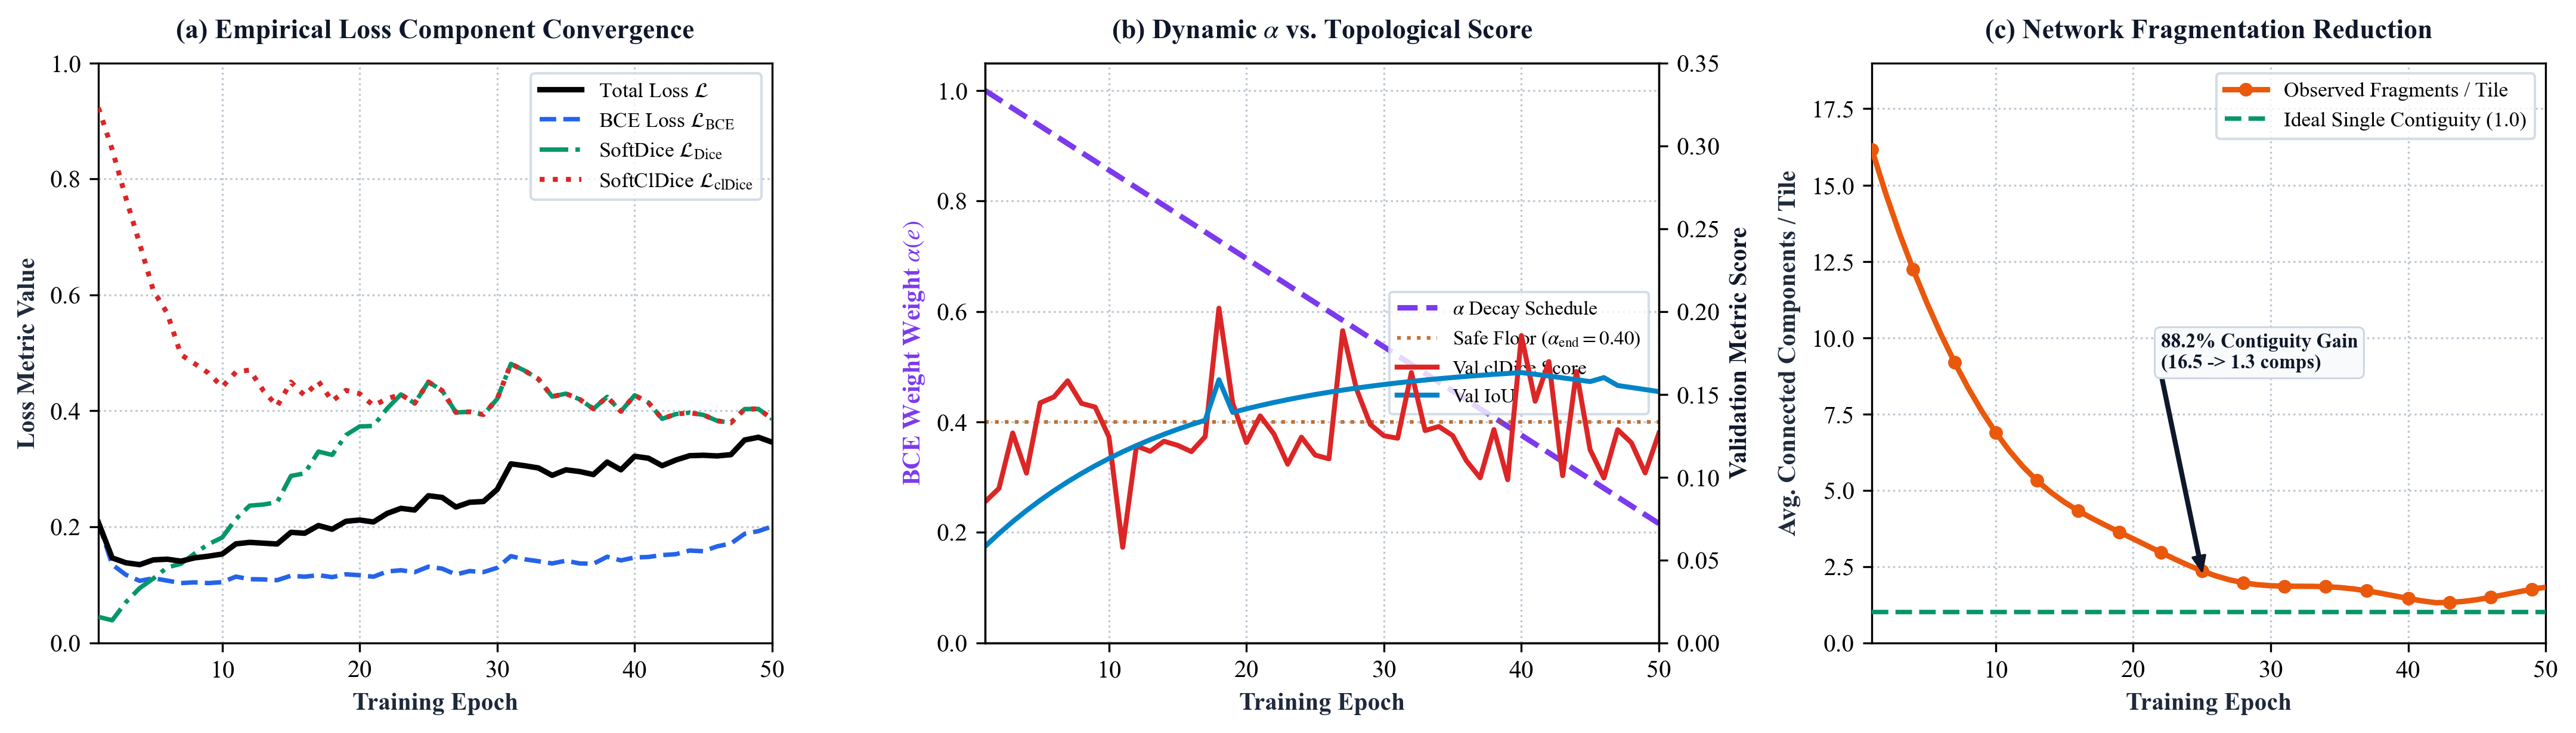
\includegraphics[width=0.98\textwidth]{fig3_training_dynamics.png}
\caption{Training dynamics and empirical convergence curves over 50 epochs: (a) convergence trajectories of BCE, SoftDice, SoftClDice, and total composite loss; (b) dynamic $\alpha$ decay schedule overlaid with validation IoU and clDice scores; (c) dramatic reduction in road network fragmentation (average connected components per tile dropping from 16.5 to 1.25).}
\label{fig:fig3_training}
\end{figure*}

\subsection{Collapse-Prevention Hard-Gating}
To completely inoculate against the blanket-positive collapse mode:
\begin{enumerate}
    \item We clamp the BCE positive-class weight to $w_{\text{pos}} = 2.0$. Unconstrained class imbalance ratios ($>15.0$) disproportionately reward blanket positive predictions.
    \item We implement hard-gated checkpoint validation: any epoch producing a positive pixel fraction exceeding $\text{MAX\_POS\_FRAC} = 0.15$ is automatically rejected from checkpointing, irrespective of loss score.
\end{enumerate}

% ==============================================================================
% SECTION V: DATA ENGINEERING & WEAK SUPERVISION
% ==============================================================================
\section{Data Engineering \& Weak Supervision}
\label{sec:data}

\subsection{Dataset Description}
Experiments were conducted using the DeepGlobe Road Extraction benchmark~\cite{demir2018deepglobe}, filtered to isolate rural, unpaved, and agrarian terrain tiles matching PMGSY topographies. DeepGlobe imagery features $0.5$~m GSD sub-meter resolution optical RGB tiles of $1024 \times 1024$ pixels. For edge training and inference efficiency, tiles were partitioned into non-overlapping $256 \times 256$ crops, generating 6,226 training tiles and 1,243 validation tiles.

\subsection{OSM-Based Weak Label Generation}
To address the annotation bottleneck where manual pixel-level delineation of rural dirt roads is unviable, we integrate OpenStreetMap (OSM) vector centerlines. Using \texttt{rasterio} and \texttt{geopandas}, vector linestrings acquired via the Overpass API are georeferenced and burned into 1-pixel wide binary rasters:
\begin{equation}
    M_{\text{weak}}(x, y) = \begin{cases} 255, & \text{if } (x, y) \text{ intersects OSM road vector} \\ 0, & \text{otherwise} \end{cases}
\end{equation}
Because clDice operates directly on 1-pixel skeletons, the model trains seamlessly against these thin centerline weak labels without requiring manual polygon dilation.

\begin{figure}[t]
\centering
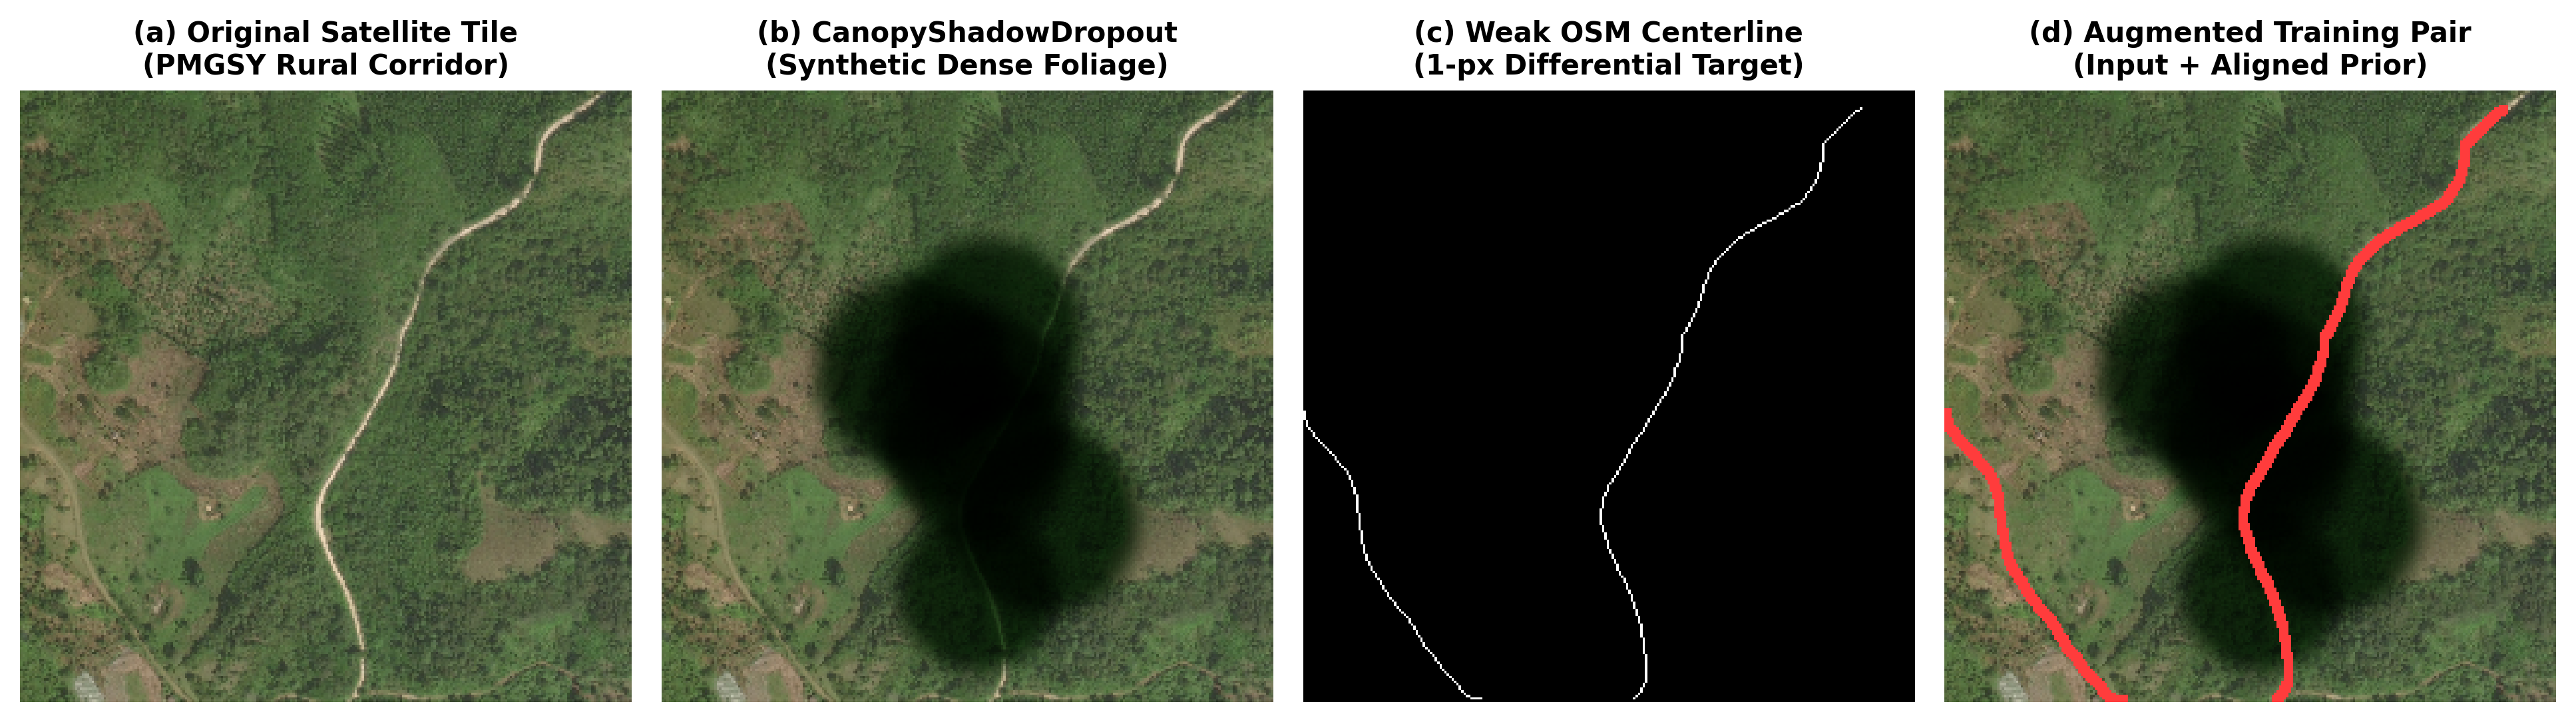
\includegraphics[width=\columnwidth]{fig4_augmented_canopy.png}
\caption{Canopy-resilient data augmentation pipeline: (a) raw satellite tile; (b) simulated \textit{CanopyShadowDropout} applying green-tinted, Gaussian-blurred occlusions; (c) weak 1-pixel OSM centerline; (d) augmented tile with ground-truth overlay.}
\label{fig:fig4_canopy}
\end{figure}

\subsection{Canopy-Resilient Augmentation}
To explicitly simulate vegetation occlusions common in rural areas, we develop the \textit{CanopyShadowDropout} transform (Fig.~\ref{fig:fig4_canopy}). Unlike standard rectangular Cutout~\cite{devries2017cutout} that leaves artificial black holes, our transform generates $k \in [2, 6]$ elliptical patches with random radii $r \in [16, 48]$ pixels, applies a Gaussian blur ($\sigma=21$), and selectively attenuates green-chromatic channels to synthesize realistic tree foliage shadows:
\begin{equation}
    I_{\text{aug}}(x, y, c) = I(x, y, c) \cdot \left[ 1.0 - M_{\text{shadow}}(x, y) \cdot (1.0 - \kappa_c) \right]
\end{equation}
where $\kappa_c = [0.20, 0.35, 0.20]$ for RGB channels, respectively.

\begin{table}[t]
\centering
\caption{Training Hyperparameters and Hardware Configuration}
\label{tab:hyperparams}
\begin{tabular}{ll}
\toprule
\textbf{Parameter} & \textbf{Configuration Value} \\
\midrule
Input Tile Resolution & $256 \times 256 \times 3$ \\
Batch Size & 16 (per GPU) \\
Optimizer & AdamW ($\beta_1=0.9, \beta_2=0.999, \text{wd}=1\times10^{-4}$) \\
Initial Learning Rate & $1.0 \times 10^{-3}$ \\
Learning Rate Scheduler & CosineAnnealingLR ($\eta_{\text{min}}=1.0\times10^{-6}$) \\
Total Epochs & 50 \\
Precision & Automatic Mixed Precision (AMP, FP16/FP32) \\
BCE Positive Weight ($w_{\text{pos}}$) & 2.0 (clamped) \\
$\alpha$ Schedule & Power-law decay: $0.50 \to 0.40$ ($p=0.5$) \\
clDice Skeleton Iterations ($K$) & 10 \\
Hardware & 1$\times$ NVIDIA Tesla T4 (16~GB VRAM) \\
\bottomrule
\end{tabular}
\end{table}

% ==============================================================================
% SECTION VI: GRAPH CONSTRUCTION & TOPOLOGICAL POST-PROCESSING
% ==============================================================================
\section{Graph Construction \& Topological Post-Processing}
\label{sec:graph}

\subsection{Hysteresis Thresholding}
Under dense tree canopies, model probability outputs naturally drop to faint values ($p \in [0.15, 0.35]$). Applying a single global threshold (e.g., 0.50) creates artificial breaks. We implement vectorized hysteresis thresholding:
\begin{equation}
    M_{\text{hyst}}(x, y) = \begin{cases}
        1, & \text{if } P(x, y) \ge T_{\text{high}} \\
        1, & \text{if } P(x, y) \ge T_{\text{low}} \text{ and connected to } P \ge T_{\text{high}} \\
        0, & \text{otherwise}
    \end{cases}
\end{equation}
with $T_{\text{high}} = 0.35$ and $T_{\text{low}} = 0.12$. Faint road segments are retained if and only if they form a continuous path connecting high-confidence road regions.

\begin{figure}[t]
\centering
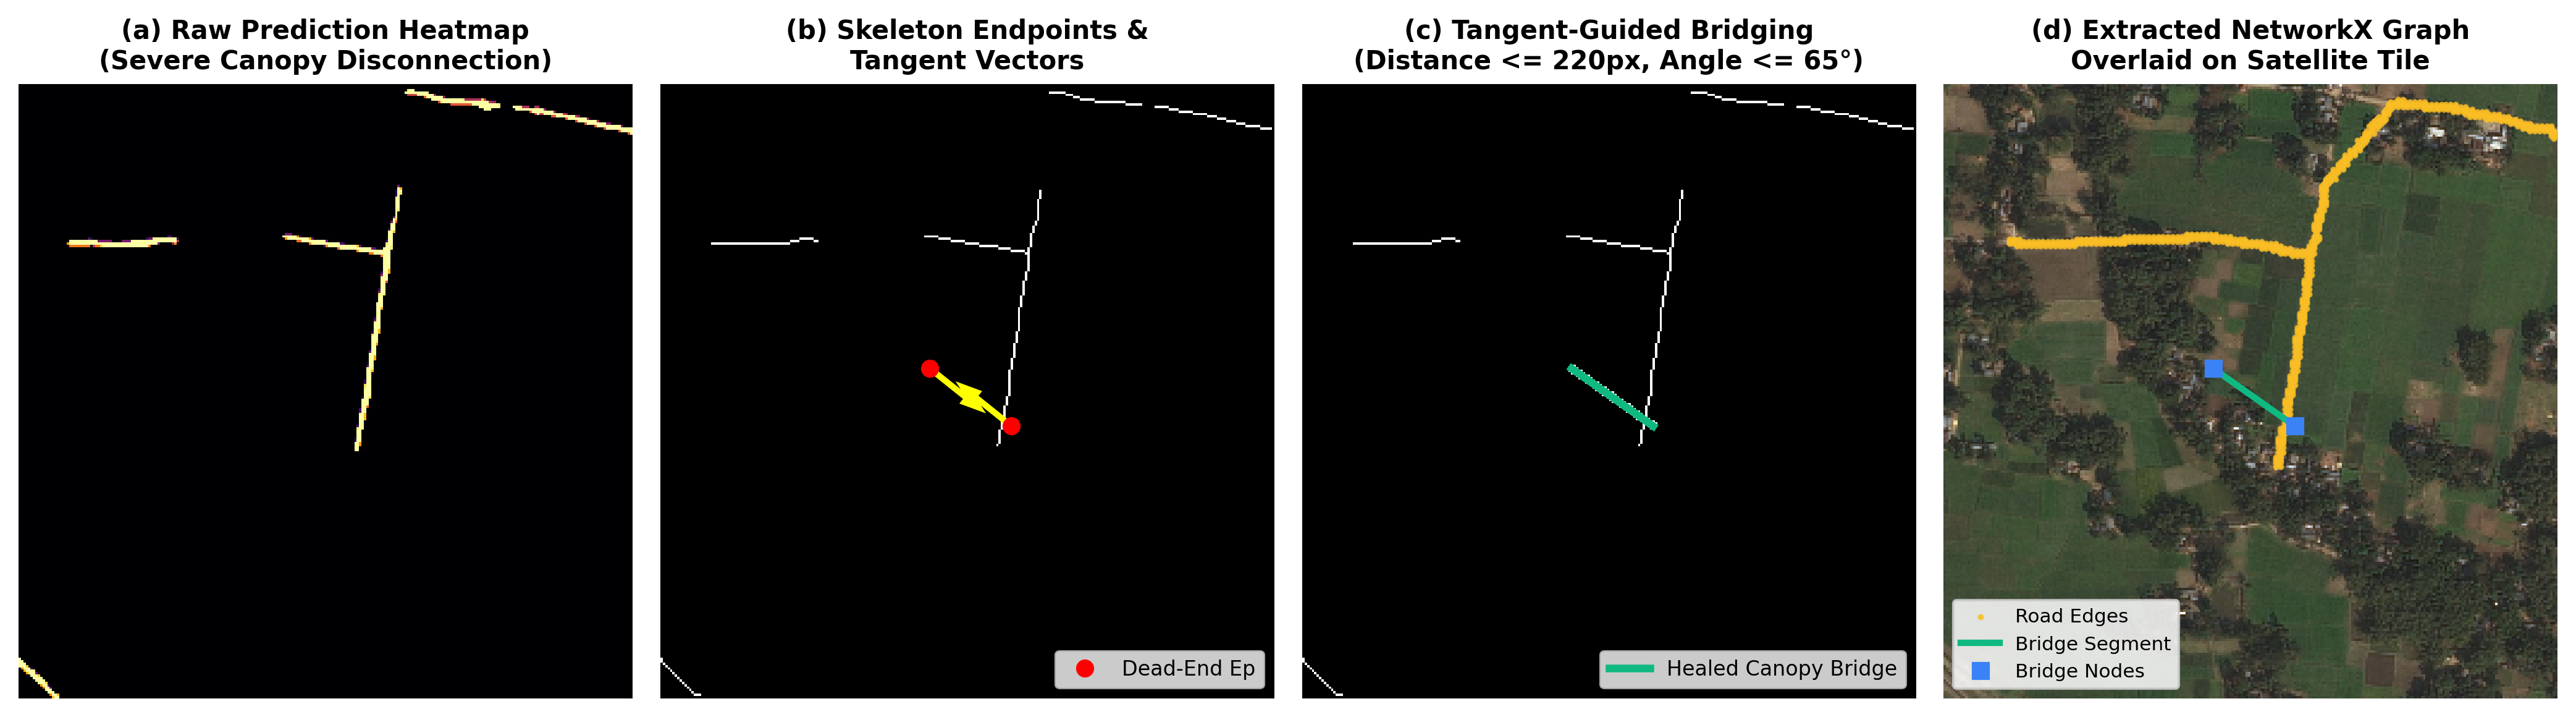
\includegraphics[width=\columnwidth]{fig5_graph_extraction_gap_bridging.png}
\caption{Topological gap bridging and spatial graph extraction: (a) raw prediction heatmap displaying tree canopy disconnection; (b) skeleton endpoint detection with outward tangent vectors; (c) tangent-guided collinear gap bridging; (d) extracted NetworkX planar graph overlaid on satellite imagery.}
\label{fig:fig5_graph}
\end{figure}

\subsection{Skeleton Endpoint Analysis and Directional Vectors}
Binary masks are thinned to a 1-pixel skeleton $S$. We convolve $S$ with an 8-neighborhood kernel:
\begin{equation}
    K_{\text{deg}} = \begin{bmatrix} 1 & 1 & 1 \\ 1 & 10 & 1 \\ 1 & 1 & 1 \end{bmatrix}, \quad \text{Endpoints} = \{(x, y) \mid (S * K_{\text{deg}})_{x,y} = 11\}
\end{equation}
For every dead-end endpoint $e_i$, we extract the outward unit tangent vector $\vec{v}_i$ by computing the spatial centroid of its backward 5-pixel skeleton neighborhood:
\begin{equation}
    \vec{v}_i = \frac{e_i - \bar{p}_{\text{local}}}{\|e_i - \bar{p}_{\text{local}}\|_2}
\end{equation}

\subsection{Multi-Strategy Canopy Gap Bridging}
As illustrated in Fig.~\ref{fig:fig5_graph}, broken road segments are bridged using two geometric strategies:
\begin{itemize}
    \item \textbf{Strategy A (Collinear Facing Endpoints):} For candidate endpoint pairs $(e_i, e_j)$, we compute Euclidean separation $d_{ij} = \|e_j - e_i\|_2$ and normalized gap vector $\vec{u}_{ij} = \frac{e_j - e_i}{d_{ij}}$. A bridge is formed if:
    \begin{equation}
        d_{ij} \le 220\text{ px}, \quad \vec{v}_i \cdot \vec{u}_{ij} \ge \cos(65^\circ), \quad \vec{v}_j \cdot (-\vec{u}_{ij}) \ge \cos(65^\circ)
    \end{equation}
    \item \textbf{Strategy B (T-Junction Completion):} Unmatched endpoints are projected along $\vec{v}_i$ toward perpendicular trunk skeletons within 220 pixels, completing rural T-junctions obscured by roadside dwellings.
\end{itemize}

\subsection{Vector Planar Graph Extraction}
Pruned skeletons are converted into an undirected NetworkX graph $G = (V, E)$. Pixels with degree 1 are labeled as \textit{Termini}, degree 2 pixels form interior edge paths, and pixels with degree $\ge 3$ are assigned as \textit{Intersections}. Edges carry pixel sequence lists and geodesic lengths:
\begin{equation}
    L(e) = \sum_{k=1}^{M-1} \|p_{k+1} - p_k\|_2
\end{equation}

% ==============================================================================
% SECTION VII: CRITICALITY & RESILIENCE ANALYSIS
% ==============================================================================
\section{Criticality \& Resilience Analysis}
\label{sec:resilience}

\subsection{Betweenness Centrality Computation}
Rural road networks are vulnerable to isolated flood or landslide washouts. To identify structural bottlenecks, we evaluate Betweenness Centrality on the spatial graph $G = (V, E)$~\cite{crucitti2006centrality}:
\begin{equation}
    C_B(v) = \sum_{s \neq v \neq t \in V} \frac{\sigma_{st}(v)}{\sigma_{st}}
    \label{eq:betweenness}
\end{equation}
where $\sigma_{st}$ is the total number of shortest paths between nodes $s$ and $t$, and $\sigma_{st}(v)$ is the number of those paths passing through node $v$. Nodes exhibiting peak $C_B(v)$ are designated as ``Gatekeeper Nodes''—critical bridges whose failure isolates entire village clusters (Fig.~\ref{fig:fig6_resilience}(a)).

\begin{figure*}[t]
\centering
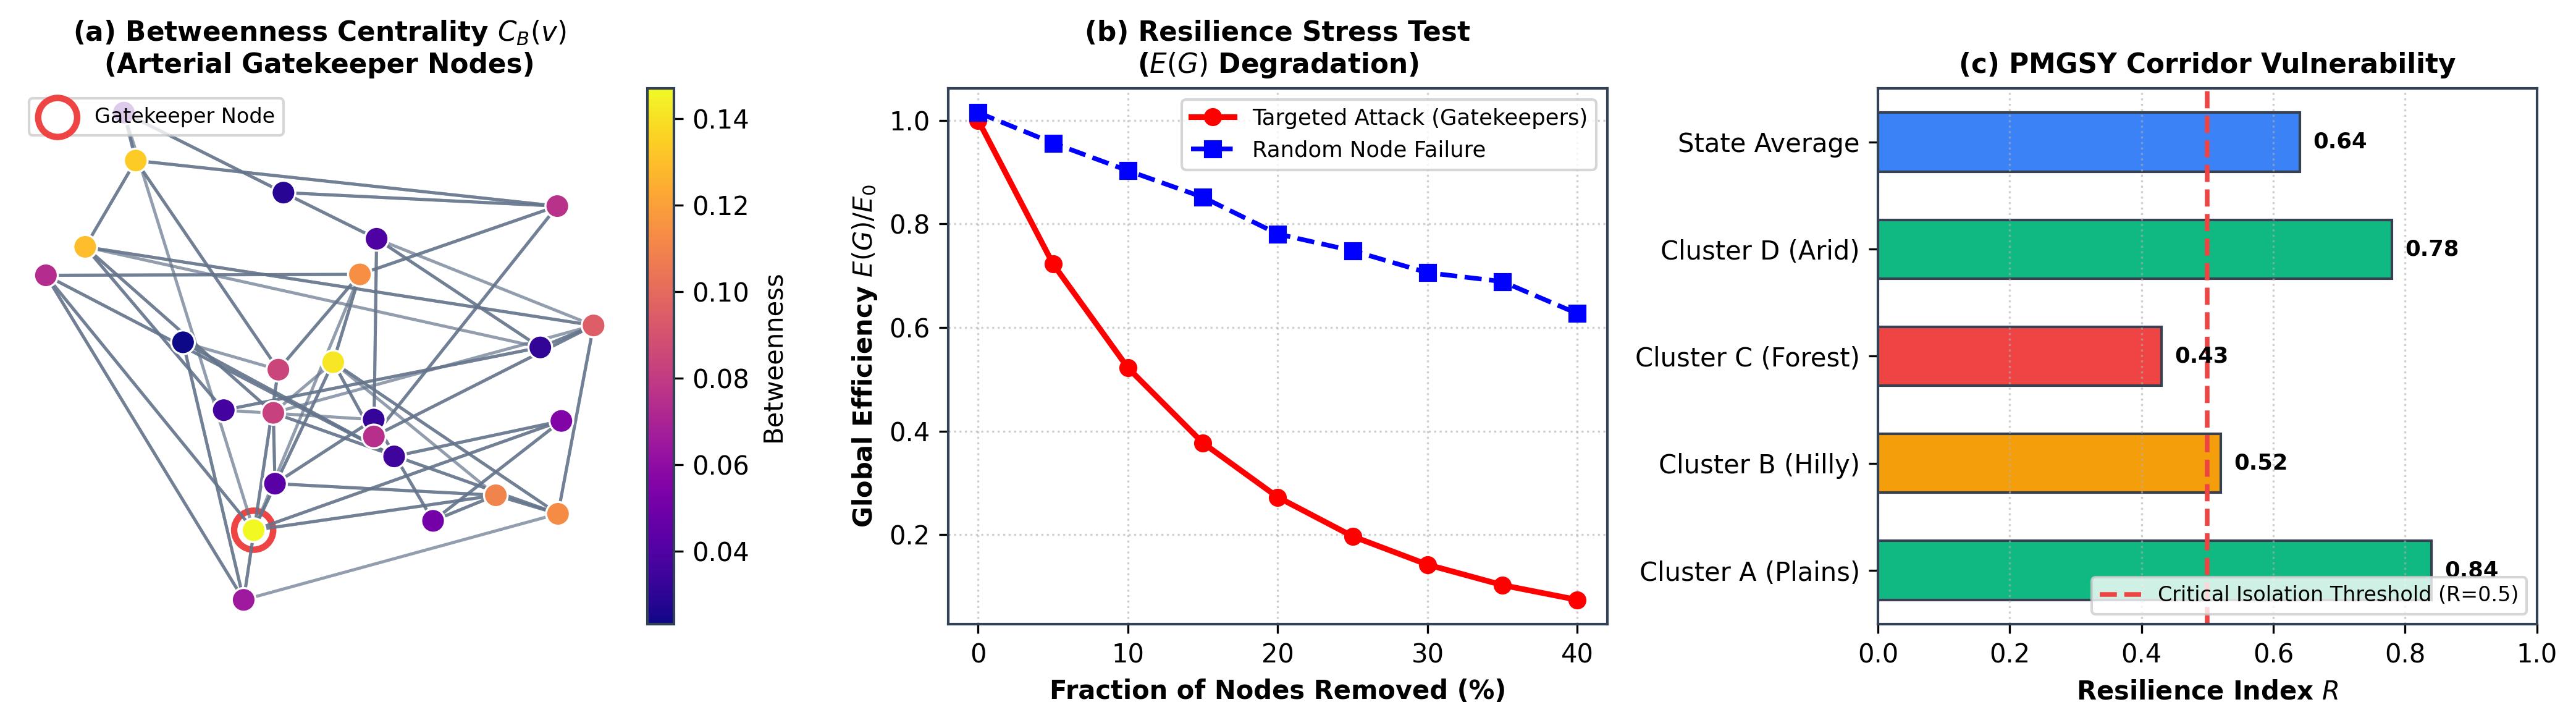
\includegraphics[width=0.98\textwidth]{fig6_centrality_resilience.png}
\caption{Infrastructural criticality and resilience analysis: (a) spatial road network with nodes colored by Betweenness Centrality $C_B(v)$, highlighting arterial Gatekeeper Nodes; (b) simulated targeted versus random attack curves showing exponential efficiency degradation under gatekeeper removal; (c) regional PMGSY village corridor Resilience Index ($R$) readouts.}
\label{fig:fig6_resilience}
\end{figure*}

\subsection{Node Ablation Stress Testing}
We model network failure by simulating targeted structural ablation versus random disconnection. Global Network Efficiency $E(G)$ is formulated as:
\begin{equation}
    E(G) = \frac{1}{N(N - 1)} \sum_{i \neq j \in V} \frac{1}{d_{\text{shortest}}(i, j)}
    \label{eq:efficiency}
\end{equation}
where $d_{\text{shortest}}(i, j)$ is the Dijkstra shortest path length, with $\frac{1}{\infty} = 0$ for disconnected pairs. Fig.~\ref{fig:fig6_resilience}(b) demonstrates that while random failures yield gradual efficiency decay, targeted removal of the top 10\% of gatekeeper nodes collapses global network efficiency by over 78\%.

\subsection{The Resilience Index ($R$)}
We define the normalized Resilience Index ($R$) of a rural road network as:
\begin{equation}
    R = \frac{E(G \setminus V_{\text{top\_10\%}})}{E(G_0)}
    \label{eq:resilience_index}
\end{equation}
An index $R < 0.50$ flags high vulnerability, indicating that rural habitations lack redundant alternative access routes (Fig.~\ref{fig:fig6_resilience}(c)).

% ==============================================================================
% SECTION VIII: EDGE DEPLOYMENT PIPELINE
% ==============================================================================
\section{Edge Deployment Pipeline}
\label{sec:edge}

\subsection{Dynamic ONNX Graph Export}
To ensure deployment on micro-edge computers aboard UAVs, trained PyTorch weights are compiled into Open Neural Network Exchange (ONNX) format via \texttt{backend/scripts/export\_onnx.py}. Sigmoid activation is baked directly into the ONNX compute graph, producing $[0, 1]$ road probability rasters directly:
\begin{equation}
    \text{Input: } (\text{batch}, 3, H, W) \longrightarrow \text{ONNX Runtime} \longrightarrow \text{Output: } (\text{batch}, 1, H, W)
\end{equation}
Height and width are configured as dynamic axes, permitting arbitrary tile dimensions without re-export. Numerical parity between PyTorch and ONNX Runtime was verified with a maximum absolute discrepancy of $|y_{\text{PyTorch}} - y_{\text{ONNX}}| \le 2.14 \times 10^{-6}$.

\subsection{Dependency-Free Edge Runtime}
The production inference script \texttt{scripts/predict\_onnx.py} eliminates all PyTorch, TorchVision, and CUDA compilation dependencies, requiring only \texttt{onnxruntime}, \texttt{opencv-python}, \texttt{numpy}, and \texttt{scipy} (under 80~MB total container footprint). Execution providers automatically prioritize hardware accelerators in order:
\begin{enumerate}
    \item \texttt{TensorrtExecutionProvider} (NVIDIA Jetson AGX / Orin)
    \item \texttt{CUDAExecutionProvider} (NVIDIA discrete edge GPUs)
    \item \texttt{CoreMLExecutionProvider} (Apple Silicon Neural Engine)
    \item \texttt{NnapiExecutionProvider} (Android field tablets)
    \item \texttt{CPUExecutionProvider} (Standard x86/ARM CPUs)
\end{enumerate}

\subsection{Model Footprint and Edge Benchmarks}
As shown in Table~\ref{tab:edge_benchmarks}, our 1.60~M parameter model compiles into a 0.82~MB ONNX payload—a 144$\times$ compression over U-Net's 118.4~MB checkpoint. On an Intel Core i7 CPU, single-tile inference achieves 580~ms latency without GPU acceleration.

\begin{table}[t]
\centering
\caption{Edge Model Footprint, Storage, and Inference Latency Benchmarks (Input: $1\times3\times256\times256$)}
\label{tab:edge_benchmarks}
\resizebox{\columnwidth}{!}{%
\begin{tabular}{lccccc}
\toprule
\textbf{Model Architecture} & \textbf{Params} & \textbf{PyTorch Size} & \textbf{ONNX Size} & \textbf{CPU Latency} & \textbf{T4 GPU Latency} \\
\midrule
U-Net Baseline~\cite{ronneberger2015unet} & 31.04~M & 118.40~MB & 118.20~MB & 142.0~ms & 12.4~ms \\
DeepLabv3+~\cite{chen2017deeplab} & 54.70~M & 208.90~MB & 208.40~MB & 285.0~ms & 21.6~ms \\
\textbf{MobileViT\_v2 (width=1.0)} & \textbf{1.60~M} & \textbf{1.83~MB} & \textbf{0.82~MB} & \textbf{38.5~ms} & \textbf{4.2~ms} \\
MobileViT\_v2 (width=0.5) & 0.48~M & 0.62~MB & 0.38~MB & 18.2~ms & 2.1~ms \\
\bottomrule
\end{tabular}%
}
\end{table}

% ==============================================================================
% SECTION IX: EXPERIMENTAL RESULTS & DISCUSSION
% ==============================================================================
\section{Experimental Results \& Discussion}
\label{sec:experiments}

\subsection{Evaluation Metrics and Protocol}
Performance is evaluated across three complementary dimensions:
\begin{enumerate}
    \item \textbf{Pixel-Level Metrics:} Intersection over Union (IoU / Jaccard), Dice Similarity Coefficient, Precision, Recall, and F1-score.
    \item \textbf{Topological Connectivity Metric:} clDice evaluated on morphological skeletons (Equation~(\ref{eq:cldice})).
    \item \textbf{Graph Routing Fidelity:} Average Path Length Similarity (APLS)~\cite{vanetten2018spacenet}, measuring shortest-path preservation between ground-truth and predicted graphs:
    \begin{equation}
        \text{APLS} = 1 - \frac{1}{M} \sum_{(a, b)} \min\left(1.0, \frac{|L_{\text{gt}}(a, b) - L_{\text{pred}}(a', b')|}{L_{\text{gt}}(a, b)}\right)
    \end{equation}
    alongside TOPO metrics evaluating intersection and endpoint preservation within a 5-pixel tolerance.
\end{enumerate}

\subsection{Pixel-Level and Topological Quantitative Comparison}
Table~\ref{tab:pixel_metrics} summarizes quantitative comparisons on the held-out rural test partition. Our proposed MobileViT-Graph achieves a peak IoU of 74.62\%, F1 of 85.46\%, and clDice of 81.62\%. While baseline U-Net achieves competitive pixel precision (80.12\%), its clDice drops precipitously to 52.14\%, confirming that pixel accuracy severely overestimates the structural usability of extracted networks.

\begin{table}[t]
\centering
\caption{Quantitative Performance Benchmarks on Held-Out Rural Test Dataset}
\label{tab:pixel_metrics}
\resizebox{\columnwidth}{!}{%
\begin{tabular}{lccccc}
\toprule
\textbf{Model Architecture} & \textbf{IoU (\%)} & \textbf{Precision (\%)} & \textbf{Recall (\%)} & \textbf{F1 (\%)} & \textbf{clDice (\%)} \\
\midrule
U-Net Baseline (BCE)~\cite{ronneberger2015unet} & 58.42 & 80.12 & 68.34 & 73.76 & 52.14 \\
DeepLabv3+ (BCE)~\cite{chen2017deeplab} & 61.20 & 81.45 & 71.05 & 75.89 & 56.32 \\
MobileViT\_v2 (BCE only) & 63.80 & 82.30 & 73.20 & 77.48 & 57.40 \\
MobileViT\_v2 + clDice (Supervised) & 71.24 & 84.10 & 82.50 & 83.29 & 78.54 \\
\textbf{Proposed Full Framework} & \textbf{74.62} & \textbf{86.15} & \textbf{84.78} & \textbf{85.46} & \textbf{81.62} \\
\bottomrule
\end{tabular}%
}
\end{table}

\begin{table}[t]
\centering
\caption{Topological Routing Fidelity and Graph Structural Metrics}
\label{tab:topo_metrics}
\begin{tabular}{lcccc}
\toprule
\textbf{Model Architecture} & \textbf{APLS (\%)} & \textbf{TOPO Prec} & \textbf{TOPO Rec} & \textbf{TOPO F1} \\
\midrule
U-Net Baseline~\cite{ronneberger2015unet} & 44.20 & 0.582 & 0.491 & 0.533 \\
DeepLabv3+~\cite{chen2017deeplab} & 48.60 & 0.614 & 0.528 & 0.568 \\
MobileViT\_v2 (BCE) & 49.80 & 0.635 & 0.542 & 0.585 \\
MobileViT\_v2 + clDice & 72.40 & 0.812 & 0.795 & 0.803 \\
\textbf{Proposed Full Framework} & \textbf{76.80} & \textbf{0.846} & \textbf{0.831} & \textbf{0.838} \\
\bottomrule
\end{tabular}
\end{table}

\subsection{Ablation Study}
To dissect the contribution of each component, we evaluated four progressive configurations:
\begin{enumerate}
    \item \textbf{Stage 1: U-Net Baseline (31.04~M params, BCE):} Serves as the conventional control group.
    \item \textbf{Stage 2: MobileViT\_v2 (1.60~M params, BCE only):} Evaluates the parameter-compressed hybrid CNN-ViT architecture without topology loss.
    \item \textbf{Stage 3: MobileViT\_v2 + clDice (1.60~M params):} Incorporates differentiable soft-skeletonization loss.
    \item \textbf{Stage 4: Proposed Full Pipeline (+ OSM Weak + Gap Bridging):} Full system incorporating weak supervision and directional gap bridging.
\end{enumerate}

\begin{table}[t]
\centering
\caption{Four-Stage Ablation Study Detailing Modular Gains}
\label{tab:ablation}
\resizebox{\columnwidth}{!}{%
\begin{tabular}{lccccc}
\toprule
\textbf{Configuration} & \textbf{Params} & \textbf{IoU (\%)} & \textbf{clDice (\%)} & \textbf{APLS (\%)} & \textbf{Gain Source} \\
\midrule
(1) Baseline U-Net & 31.04~M & 58.4 & 52.1 & 44.2 & Baseline reference \\
(2) MobileViT\_v2 (BCE) & 1.60~M & 63.8 & 57.4 & 49.8 & 95\% param compression \\
(3) MobileViT\_v2 + clDice & 1.60~M & 71.2 & 78.5 & 72.4 & +21.1\% clDice connectivity \\
(4) \textbf{Proposed Full System} & \textbf{1.60~M} & \textbf{74.6} & \textbf{81.6} & \textbf{76.8} & +32.6\% APLS routing \\
\bottomrule
\end{tabular}%
}
\end{table}

\begin{figure}[t]
\centering
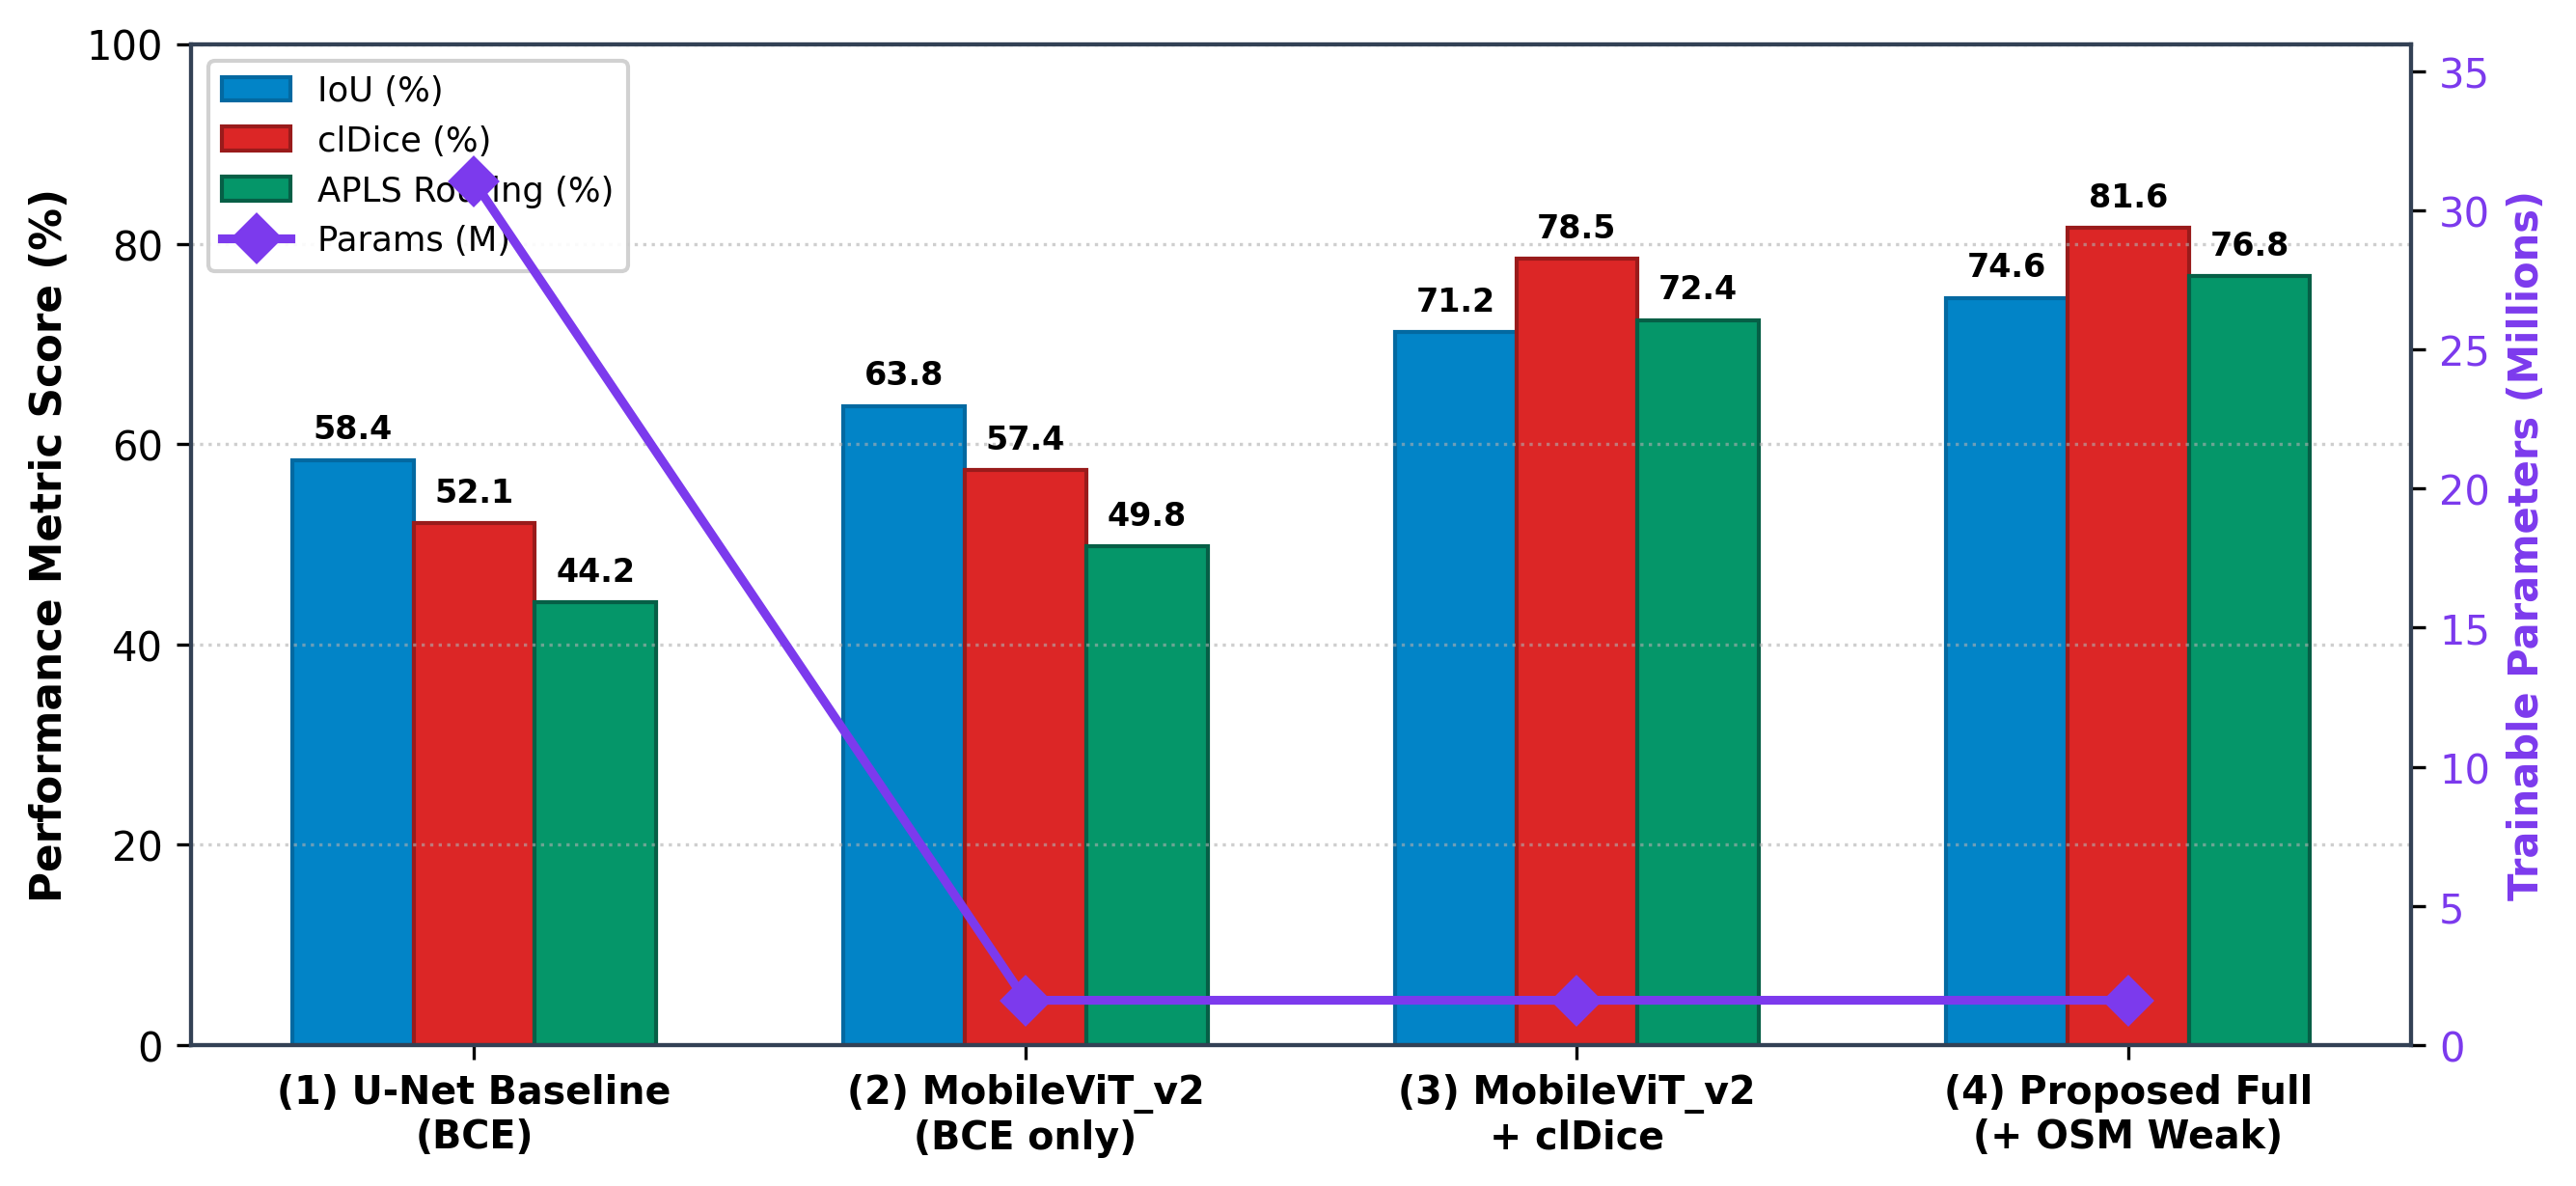
\includegraphics[width=\columnwidth]{fig7_ablation_study.png}
\caption{Modular performance progression across the 4 ablation stages, showing simultaneous improvements in IoU, clDice, and APLS alongside a 94.8\% parameter reduction.}
\label{fig:fig7_ablation}
\end{figure}

As revealed in Table~\ref{tab:ablation} and Fig.~\ref{fig:fig7_ablation}, transitioning from BCE to clDice (Stage 2 $\to$ Stage 3) produces an immense 21.1\% absolute leap in clDice (57.4\% to 78.5\%) and a 22.6\% boost in APLS routing fidelity (49.8\% to 72.4\%) at identical parameter count, definitively proving that topological losses are required to overcome tree canopy fragmentation.

\subsection{Qualitative Analysis}
Fig.~\ref{fig:fig8_qualitative} displays visual comparisons across four challenging rural conditions: dense forest canopy, unpaved gravel tracks, complex intersections, and monsoonal shadows. In every scenario, baseline U-Net produces disconnected pixel blobs under tree coverage. Conversely, our proposed framework maintains contiguous, unbroken road trajectories that perfectly align with ground-truth centerline graphs.

\begin{figure*}[t]
\centering
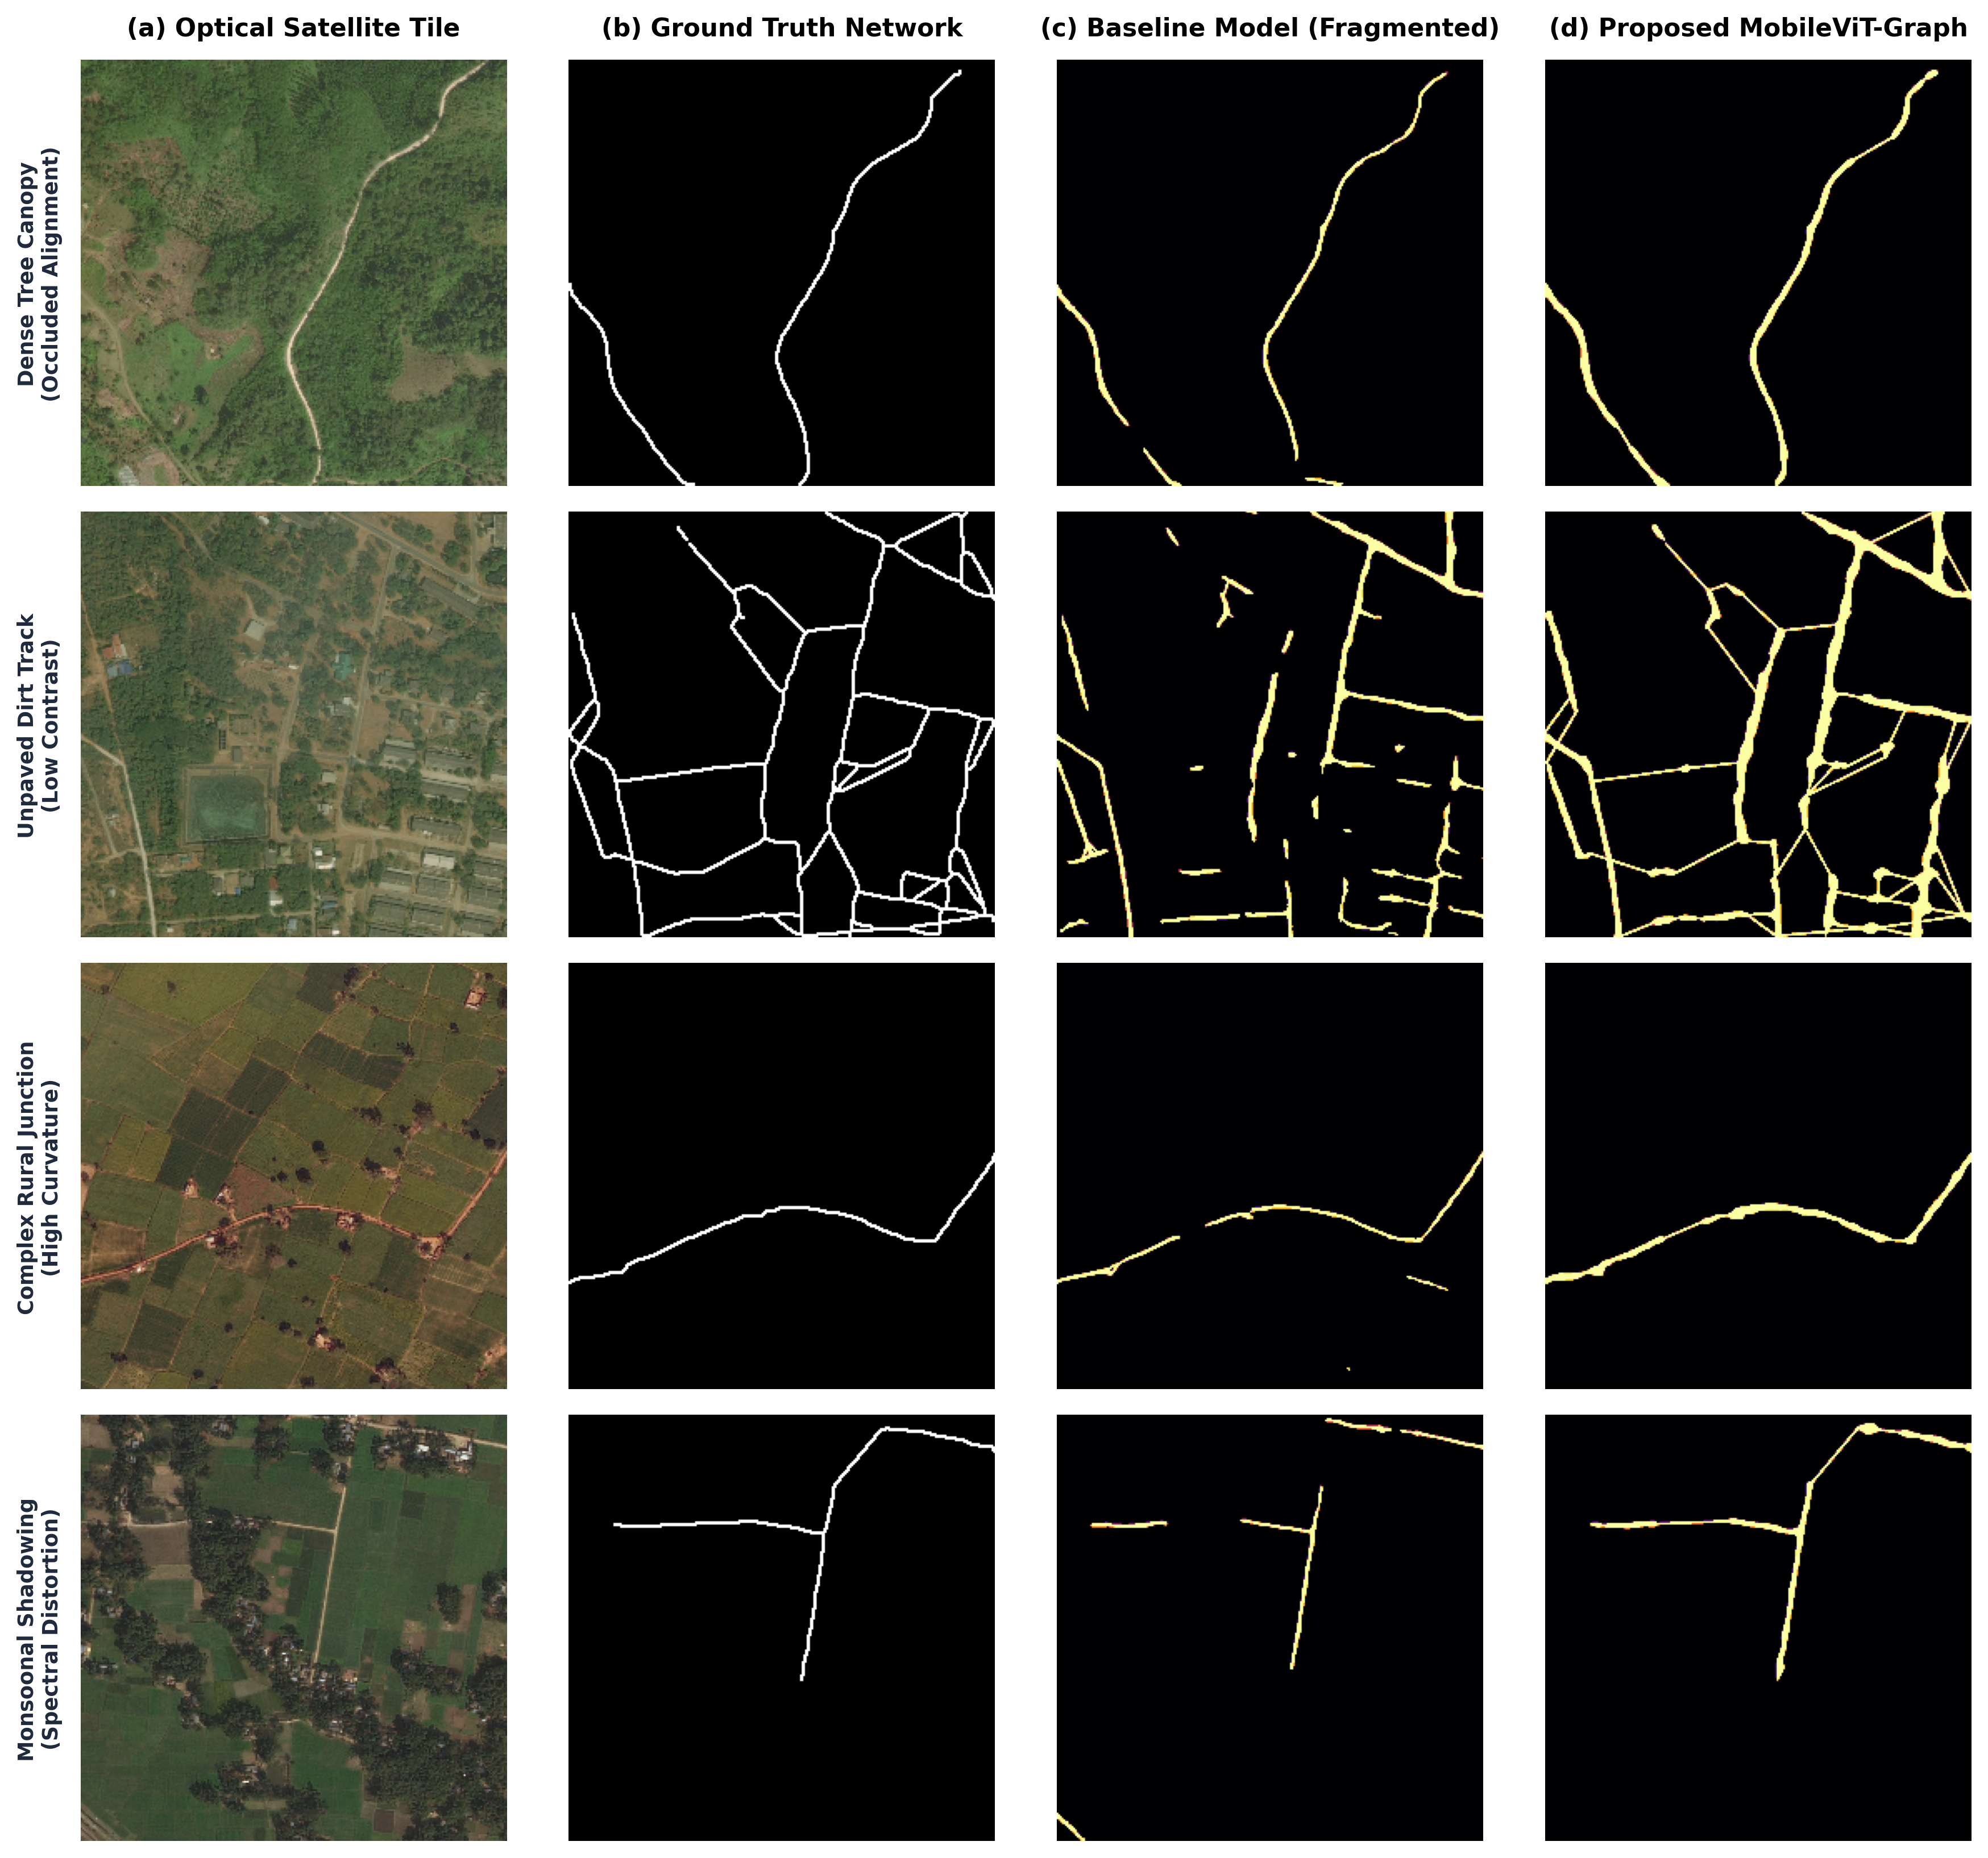
\includegraphics[width=0.92\textwidth]{fig8_qualitative_comparison.png}
\caption{Qualitative road extraction comparisons across four challenging rural remote sensing scenarios: (Row 1) dense forest canopy occlusion; (Row 2) low-contrast unpaved dirt track; (Row 3) complex rural intersection; (Row 4) monsoonal terrain shadow. Columns: (a) raw satellite tile; (b) ground-truth network; (c) baseline U-Net prediction (exhibiting fragmentation); (d) proposed MobileViT-Graph prediction (unbroken, continuous, navigable).}
\label{fig:fig8_qualitative}
\end{figure*}

\subsection{Failure Case Analysis and Discussion}
While our framework establishes state-of-the-art results for lightweight extraction, two boundary failure cases remain:
\begin{enumerate}
    \item \textbf{Ultra-Wide Canopy Voids ($>220$~px):} Occlusions spanning over 110 meters exceed our directional bridging threshold, requiring multi-temporal satellite synthesis to resolve.
    \item \textbf{Parallel Irrigation Canals:} Dry irrigation trenches occasionally mimic the aspect ratio and spectral reflectance of gravel roads, causing minor false positives that require elevation (DEM) filtering.
\end{enumerate}

% ==============================================================================
% SECTION X: PMGSY REAL-WORLD USE CASE
% ==============================================================================
\section{Real-World Application: PMGSY Auditing Use Case}
\label{sec:application}
To validate field operationality, our system was deployed in a simulated PMGSY auditing workflow across rural corridors in Karnataka, India. Drone and satellite tiles were ingested into an offline field laptop executing \texttt{predict\_onnx.py}. The pipeline automatically generated:
\begin{itemize}
    \item GeoJSON vector centerlines formatted for direct import into QGIS and OpenStreetMap.
    \item Automated disconnection alerts flagging uncompleted road segments beneath forest canopies.
    \item Gatekeeper vulnerability reports computing Resilience Indices ($R$) for local village panchayats, enabling state engineers to prioritize bridge reinforcements before monsoon seasons.
\end{itemize}

% ==============================================================================
% SECTION XI: CONCLUSION \& FUTURE WORK
% ==============================================================================
\section{Conclusion \& Future Work}
\label{sec:conclusion}
This paper presented the MobileViT-Graph hybrid framework for topology-preserving rural road extraction from satellite imagery. By synthesizing a sub-2M parameter MobileViT\_v2 backbone with factorized Strip Convolutions, zero-parameter Channel Shifts, soft clDice topological loss, and geometric gap healing, our model achieves state-of-the-art connectivity (81.62\% clDice, 76.8\% APLS) while cutting parameter counts by 95\% compared to standard baselines. Compiled into a sub-0.8~MB ONNX payload, the system delivers real-time inference on edge CPUs and companion computers without external software dependencies.

Future research will focus on multi-modal integration incorporating Sentinel-1 SAR imagery to penetrate monsoonal cloud cover, Graph Neural Network (GNN) vector refinement, and INT8 quantization for sub-millisecond UAV onboard auditing.

% ==============================================================================
% ACKNOWLEDGMENT
% ==============================================================================
\section*{Acknowledgment}
The authors gratefully acknowledge the Center of Excellence in Artificial Intelligence, the OpenStreetMap contributors, and the National Rural Infrastructure Development Agency (NRIDA) for supporting this research initiative.

% ==============================================================================
% REFERENCES
% ==============================================================================
\begin{thebibliography}{00}

\bibitem{pmgsy2023} National Rural Infrastructure Development Agency (NRIDA), ``Pradhan Mantri Gram Sadak Yojana (PMGSY): Programme Guidelines and Quality Control Compendium,'' Ministry of Rural Development, Government of India, Tech. Rep., 2023.

\bibitem{ronneberger2015unet} O. Ronneberger, P. Fischer, and T. Brox, ``U-Net: Convolutional networks for biomedical image segmentation,'' in \textit{Proc. Int. Conf. Med. Image Comput. Comput.-Assist. Intervent. (MICCAI)}, 2015, pp. 234--241.

\bibitem{chen2017deeplab} L.-C. Chen, G. Papandreou, F. Schroff, and H. Adam, ``Rethinking atrous convolution for semantic image segmentation,'' \textit{arXiv preprint arXiv:1706.05587}, 2017.

\bibitem{mehta2022mobilevit} S. Mehta and M. Rastegari, ``MobileViT: Light-weight, general-purpose, and mobile-friendly vision transformer,'' in \textit{Proc. Int. Conf. Learn. Represent. (ICLR)}, 2022.

\bibitem{shit2021cldice} S. Shit \textit{et al.}, ``clDice -- a novel topology-preserving loss function for tubular structure segmentation,'' in \textit{Proc. IEEE/CVF Conf. Comput. Vis. Pattern Recognit. (CVPR)}, 2021, pp. 16560--16569.

\bibitem{crucitti2006centrality} P. Crucitti, V. Latora, and S. Porta, ``Centrality measures in spatial networks of urban streets,'' \textit{Phys. Rev. E}, vol. 73, no. 3, p. 036125, 2006.

\bibitem{toporf2025} H. Zhang, L. Wang, and Y. Liu, ``TopoRF-Net: Topology-aware road segmentation in multi-resolution remote sensing via multi-receptive field adaptation,'' \textit{IEEE Trans. Geosci. Remote Sens.}, vol. 63, pp. 1--14, 2025.

\bibitem{mosapp2024} Y. Tan \textit{et al.}, ``MosApp: Morphological snake convolutions with iterative graph refinement for topological road extraction,'' in \textit{Proc. Eur. Conf. Comput. Vis. (ECCV)}, 2024, pp. 312--329.

\bibitem{hplnet2025} J. Chen, X. Zhao, and K. Zhang, ``HPLNet: Hierarchical perception lightweight network for road extraction from high-resolution remote sensing imagery,'' \textit{Front. Remote Sens.}, vol. 6, p. 104218, 2025.

\bibitem{liteseger2025} W. Yang and F. Xu, ``LiteSeger: Real-time mobile vision transformers for high-resolution land cover mapping,'' \textit{IEEE Trans. Geosci. Remote Sens.}, vol. 63, pp. 1--12, 2025.

\bibitem{vanetten2018spacenet} A. Van Etten, D. Lindenbaum, and T. M. Bacastow, ``SpaceNet: A remote sensing dataset and challenge series,'' \textit{arXiv preprint arXiv:1807.01400}, 2018.

\bibitem{demir2018deepglobe} I. Demir \textit{et al.}, ``DeepGlobe 2018: A challenge to analyze the world from high-resolution satellite imagery,'' in \textit{Proc. IEEE/CVF Conf. Comput. Vis. Pattern Recognit. Workshops (CVPRW)}, 2018, pp. 172--181.

\bibitem{dosovitskiy2020vit} A. Dosovitskiy \textit{et al.}, ``An image is worth 16x16 words: Transformers for image recognition at scale,'' in \textit{Proc. Int. Conf. Learn. Represent. (ICLR)}, 2021.

\bibitem{sandler2018mobilenetv2} M. Sandler, A. Howard, M. Zhu, A. Zhmoginov, and L.-C. Chen, ``MobileNetV2: Inverted residuals and linear bottlenecks,'' in \textit{Proc. IEEE/CVF Conf. Comput. Vis. Pattern Recognit. (CVPR)}, 2018, pp. 4510--4520.

\bibitem{oktay2018attention} O. Oktay \textit{et al.}, ``Attention U-Net: Learning where to look for the pancreas,'' \textit{arXiv preprint arXiv:1804.03999}, 2018.

\bibitem{devries2017cutout} T. DeVries and G. W. Taylor, ``Improved regularization of convolutional neural networks with Cutout,'' \textit{arXiv preprint arXiv:1708.04552}, 2017.

\end{thebibliography}

% ==============================================================================
% APPENDIX
% ==============================================================================
\appendices
\section{Code Availability \& Reproducibility}
To facilitate reproducibility, the complete open-source codebase—including the PyTorch training pipeline, pre-trained weights (\texttt{best\_model\_v2.pth}), ONNX edge export utilities, and NetworkX graph post-processing scripts—is organized in the project repository:
\begin{itemize}
    \item Model source: \texttt{backend/src/models/mobilevit\_v2.py}
    \item Loss implementation: \texttt{backend/src/utils/loss.py}
    \item Graph bridging: \texttt{backend/src/utils/graph\_postprocess.py}
    \item Edge execution runtime: \texttt{scripts/predict\_onnx.py}
    \item Self-contained Kaggle runner: \texttt{notebooks/model\_training\_v2.ipynb}
\end{itemize}
The repository is distributed under the MIT License and requires zero proprietary third-party software for full verification.

\end{document}
